\documentclass{article}
\input{../../../LaTex/preamble/preamble_article.tex}

\begin{comment}
    重复语句
    \subsubsection{}
    \includegraphics[width=50em,keepaspectratio]{}

    \begin{itemize}
        \item 错选:\quad
        \item 正解:\quad
        \item 总结:\quad
        \item 扩展:\quad
    \end{itemize}

\end{comment}


\title{高中物理精题集}
\author{马祥芸}

\begin{document}
\maketitle
\tableofcontents
\newpage

\section{高一}

\subsection{2022-2023年度(下)重庆八中高一期末}

\subsubsection{I-7:荷质比问题}
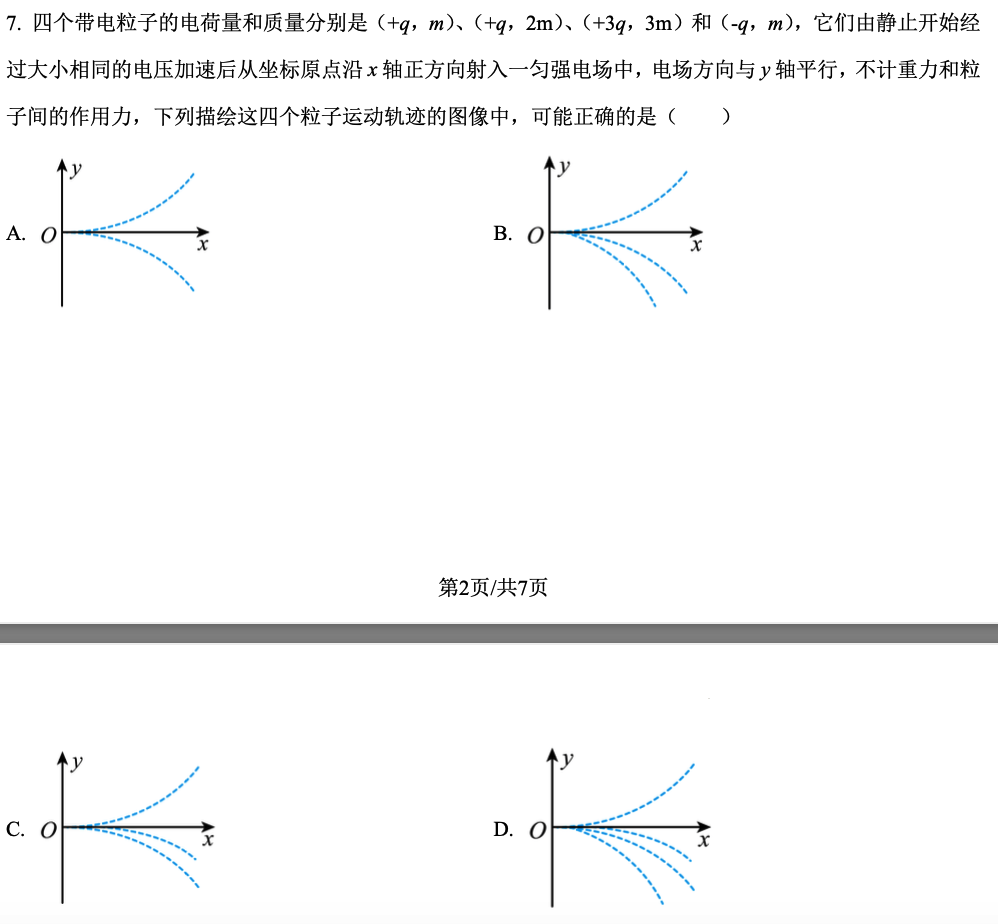
\includegraphics[width=0.95\textwidth,keepaspectratio]{./pictures/1.1-1.png}

\begin{itemize}
    \item 正解:\quad A
    \item 总结:最终要给出\textbf{轨迹方程,即$ y = f(x) $},同时注意\textbf{电荷的正负性}决定着轨迹函数所在的区间
    \item 扩展:荷质比相关题目,粒子回旋加速期、粒子速度筛选器等
\end{itemize}

\vspace{2em}

\subsubsection{II-9:不同类型的碰撞}
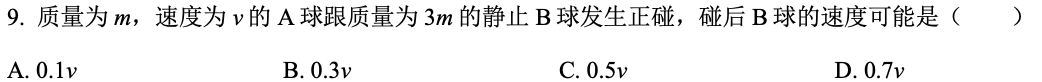
\includegraphics[width=0.95\textwidth,keepaspectratio]{./pictures/1.1-2.png}

\begin{itemize}
    \item 正解:\quad BC
    \item 总结:\quad 容易用不等式解法去求得$3m$物块的最大速度,但是无法计算最小速度。事实上$3m$物体碰
          后的\textbf{速度区间取决于碰撞过程中的动能损失程度}。
          \begin{itemize}
              \item \textbf{弹性碰撞(完全弹性碰撞)},系统机械能损失\textbf{最小},获得被碰物体\textbf{最大速度}
              \item \textbf{非弹性碰撞},系统机能损失,特点是碰后两物块\textbf{分离}
              \item \textbf{完全非弹性碰撞},碰撞后物体"粘连"  $ \lra mv_{0} = (m+3m)v^{'} $在一起,系统动能损失\textbf{最大},被碰物体获得\textbf{最小速度}。
          \end{itemize}
\end{itemize}

\vspace{2em}

\subsubsection{II-10:匀强电场下的斜射}
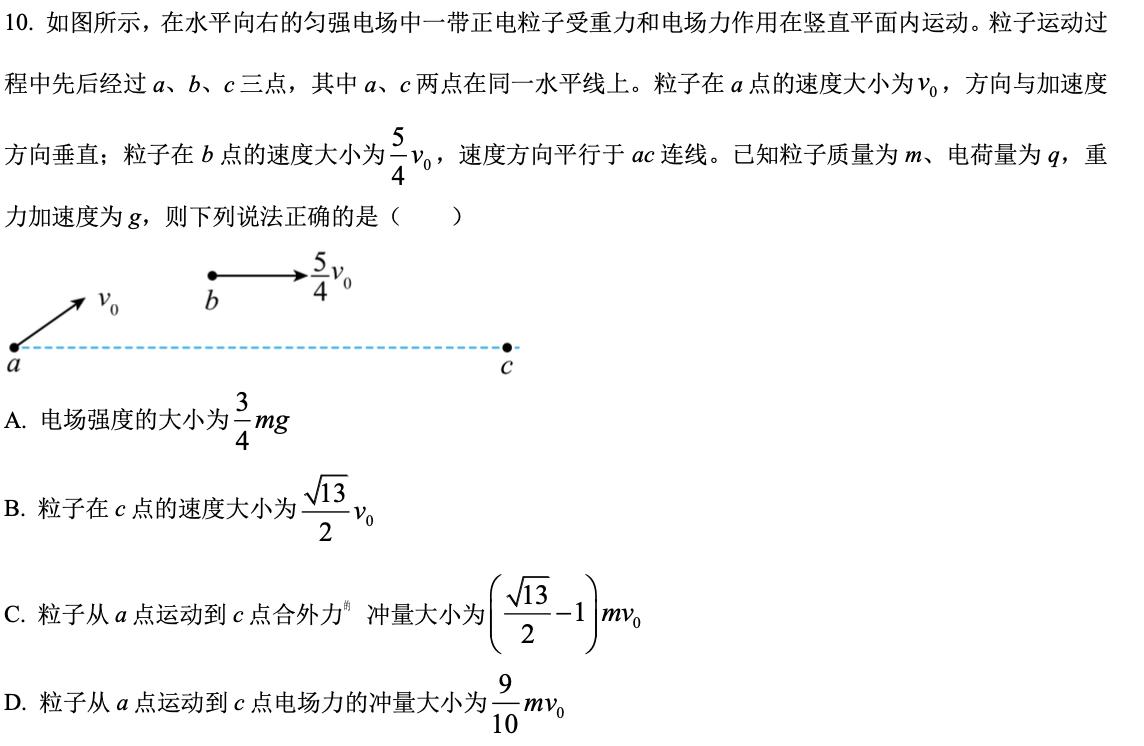
\includegraphics[width=0.95\textwidth,keepaspectratio]{./pictures/1.1-3.png}

\begin{itemize}
    \item 正解:\quad BD
    \item 总结:\quad
          \begin{itemize}
              \item 选项A \\
                    重点在于粒子在$a$点时的速度方向与加速度方向垂直。因此 \quad $b$点的速度在初速度方向的投影 \quad 与 \quad 初速度的大小一致。由此可以求得初始速度方向与水平方向的夹角$\theta$。再通过
                    相同时间内($a \rightarrow b$),重力冲量与电场力冲量下对两个方向的动量改变量,获得的两个方程消去时间$\triangle t$,得到$Eq$与$mg$的数量关系(选项$A$量纲错误)。
                    $$
                        \begin{cases}
                            mg \vdot \triangle t = m v_{0} \vdot \sin{\theta} \\
                            Eq \vdot \triangle t = \frac{5}{4} m v_{0} - m v_{0} \vdot \cos{\theta}
                        \end{cases}
                    $$

              \item 选项B \\
                    在同一水平面上,$a \rightarrow c$的时间为$a \rightarrow b$的时间的两倍(竖直运动的对称性).

                    \begin{align*}
                        mg \vdot t                     & = 2 m v_{0} \sin{\theta} \lra t = \frac{6 v_{0}}{5 g} \\
                        m v_{x} - m v_{0} \cos{\theta} & = Eq \vdot t \quad (Eq = \frac{3}{4} mg)
                    \end{align*}
                    计算合速度可以先使用水平方向上的冲量定理计算出水平方向上的速度。或者直接用动能定理(重力势能不变),计算出$a \rightarrow c$的水平距离,进而得到电场力做功。
          \end{itemize}
\end{itemize}

\vspace{2em}

\subsubsection{III-1:实验中的Q/U-t图像}
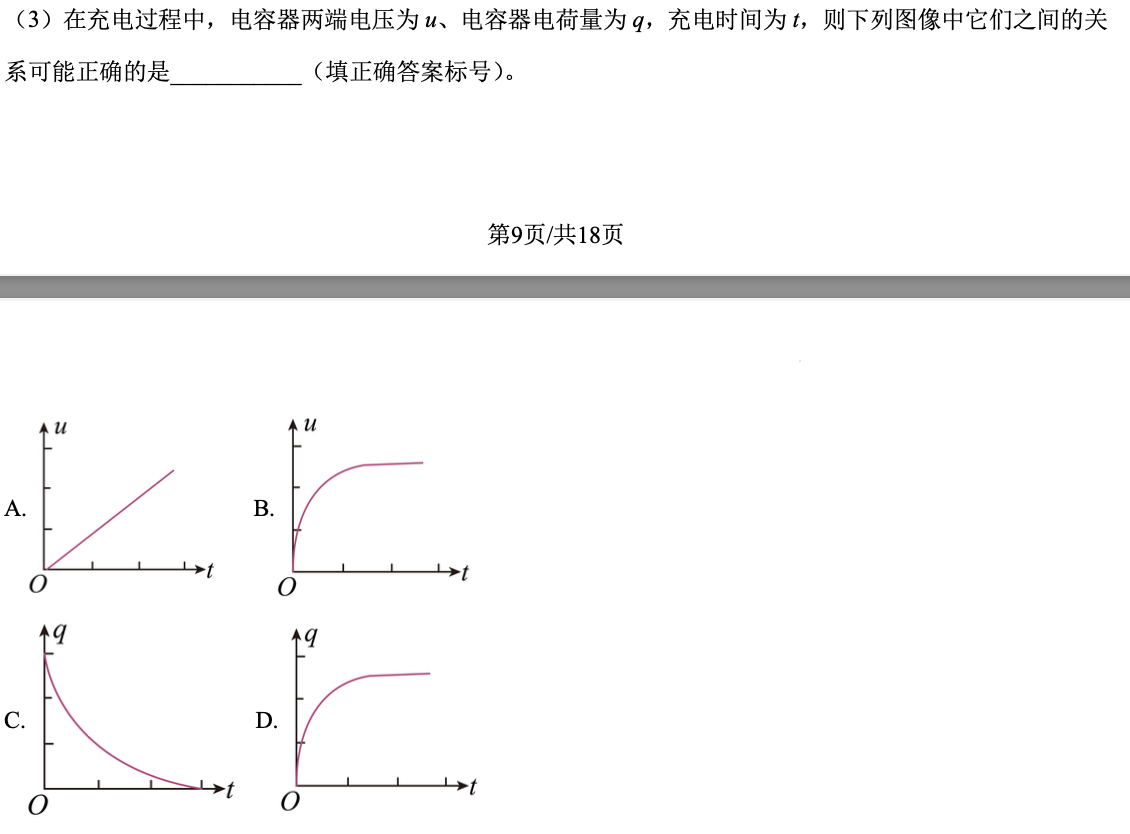
\includegraphics[width=0.95\textwidth,keepaspectratio]{./pictures/1.1-4.png}

\begin{itemize}
    \item 正解:\quad BD
    \item 总结:\quad 电容器的电压并非在一瞬间就获得,同样是电荷累计的结果
\end{itemize}

\vspace{2em}

\subsection{2022-2023育才中学期末模拟题(八)}

\subsubsection{I-4:关联体旋转运动分析}
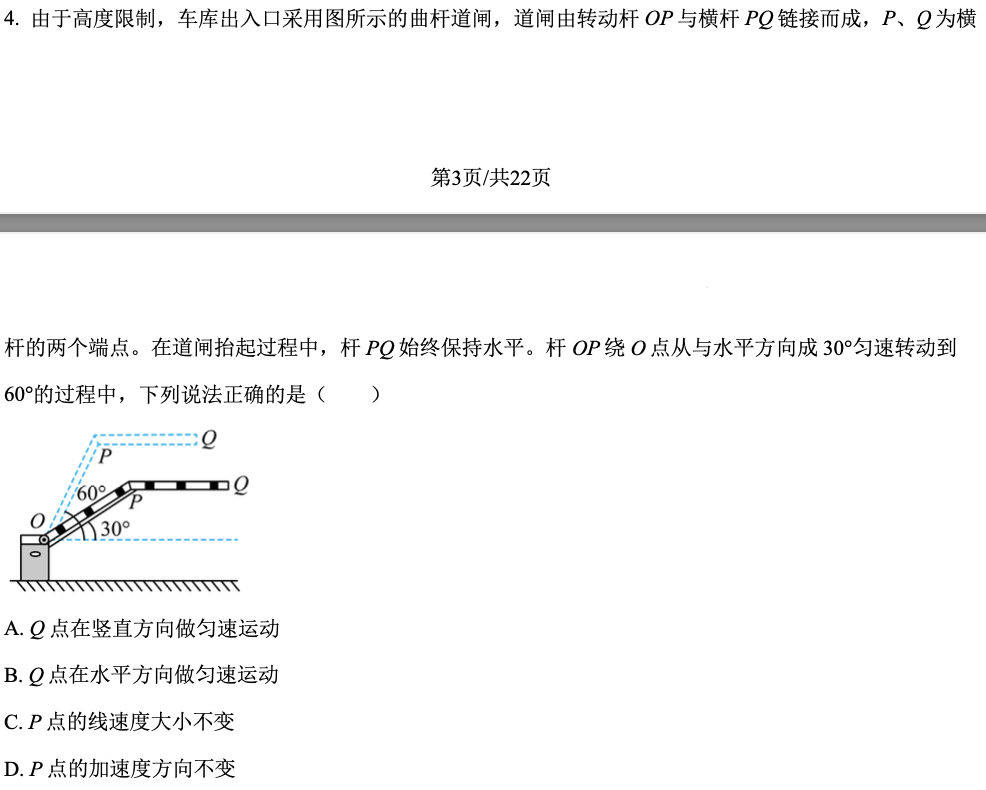
\includegraphics[width=0.95\textwidth,keepaspectratio]{./pictures/1.2-1.png}

\begin{itemize}
    \item 正解:\quad C
    \item 总结:\quad 选出正确答案并不难,本质是$\omega_{//}$
    \item 扩展:\quad 进一步思考本题,$P$点的运动为匀速圆周运动,因此其坐标$(x,y)$是可以被表示的.
          $$
              P_(x,y) = (\cos{(\omega t + \phi_{0})} , \sin{(\omega t + \phi_{0})})
          $$
          同时$Q$点的坐标也是可以被表示的,存在\textbf{几何约束},$P$到$Q$的距离为固定值线段$\overline{PQ} = L$,显然$Q$也是做匀速圆周运动
          圆心为距离圆心$O$右侧$L$处,且角速度小于$P$点.
\end{itemize}

\vspace{2em}

\subsubsection{I-7:P-t图问题}
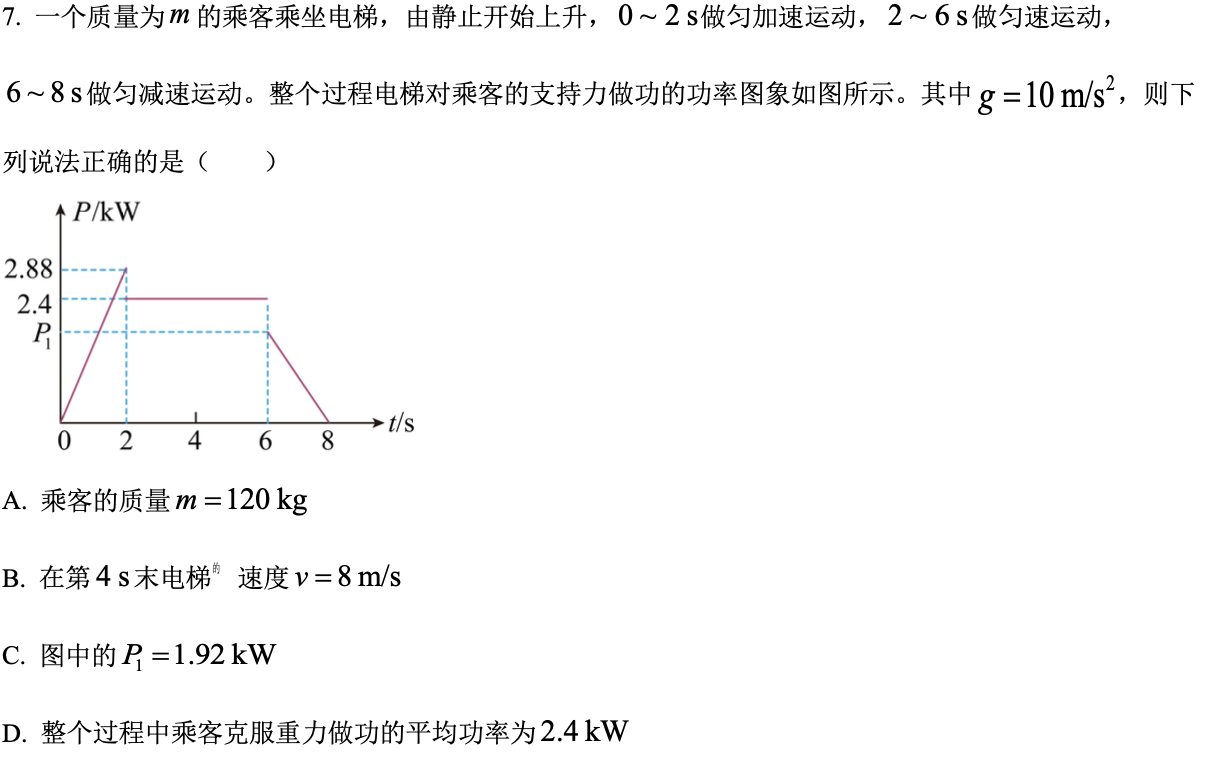
\includegraphics[width=0.95\textwidth,keepaspectratio]{./pictures/1.2-2.png}

\begin{itemize}
    \item 正解:\quad C
    \item 总结:\quad 此题分为三个阶段,同时存在一个重要的速度节点,即$t = 2s$时的速度.所列方程众多,因此理清阶段,以及要求的目标量.
          $$
              \begin{cases}
                  P_{1} = N \vdot a \vdot t = 2880 w \\
                  P_{2} = mg \vdot a \vdot t  = 2400 w
              \end{cases}
          $$
          选项$D$,可以有两种思路;第一种:计算出位移,得到重力势能做功.第二种$P-t$图所围成的面积为支持力做功的平均功率,在此过程中无
          其他力做功且初末动能均为0,因此支持力做功的平均功率等于克服重力做功的平均功率.
          $$ W = 1920j + 2880j + 9600 j \qquad t_{total} = 8s \qquad \overline{P} = \frac{W}{t_{total}} = 1.8kw $$

    \item 扩展:
          \begin{align}
              P & = N \vdot v \qquad v = v_{0} + a t \qquad v_{0} = 0 \qquad a = \frac{N-mg}{m} \\
              P & = \frac{N(N-mg)}{m} t \qquad  k = \frac{N(N-mg)}{m}
          \end{align}
\end{itemize}

\vspace{2em}

\subsubsection{II-8:水平内的碰撞+环形追及问题}
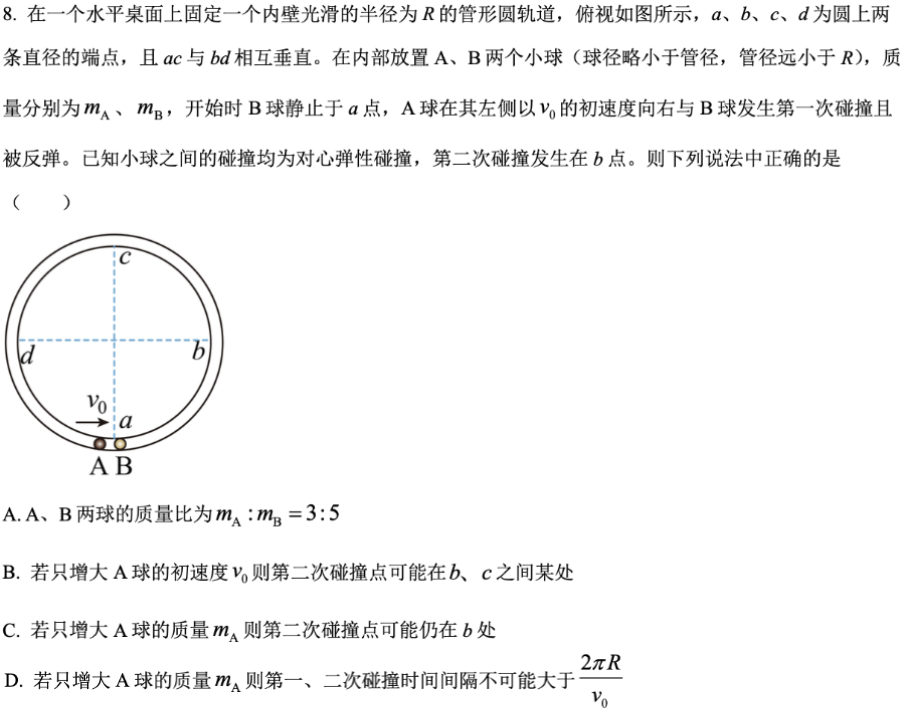
\includegraphics[width=0.95\textwidth,keepaspectratio]{./pictures/1.2-3.png}

\begin{itemize}
    \item 正解:\quad CD
    \item 总结:\quad 此物理情景发生在水平桌面上,所以不用考虑重力.所以本质是一个追及问题。同时第二次碰撞满足三个方程,第一个方程控制碰撞约束,第二、三个方程控制具体
          碰撞点
          $$
              \begin{cases}
                  v_{A} t + v_{B} t = 2 \pi R \\
                  v_{B} t  = \frac{\pi}{2}    \\
                  v_{A} t = \frac{3\pi}{2}
              \end{cases}
          $$
          选项$B$,通过前面的计算碰撞发生的时间为$t = \frac{2\pi R}{v_{0}}$ 仅仅与$v_{0}$有关,但碰后的速度也发生了变化,因此我们需要设出
          碰撞时的角度(这里取与水平线上为$\alpha$),计算出该角度的函数表达式(关于初速度质量等)
          $$
              \begin{cases}
                  v_{A} t & = (\frac{3\pi}{2} - \alpha) R           \\
                  v_{B} t & = (\frac{\pi}{2} + \alpha) R            \\
                  v_{A}   & = \frac{m_{B} - m{A}}{m_{A}+m{B}} v_{0} \\
                  v_{B}   & = \frac{2 m{A}}{m_{A}+m{B}} v_{0}
              \end{cases}
          $$

          $$
              \alpha = \frac{7 \pi}{2} \vdot \frac{m_{A} - m_{B}}{m_{A} + m_{B}}
          $$
          其碰撞点与初速度无关所以$B$错,与质量相关,当碰撞点在$b$时存在球$A$反向碰撞(题目初始情况)与球$A$同向被套圈碰撞,所以$C$对,满足$m_{A} : m_{B} = 5 : 3$
\end{itemize}

\vspace{2em}

\subsubsection{III-12:动量守恒实验-圆弧约束}
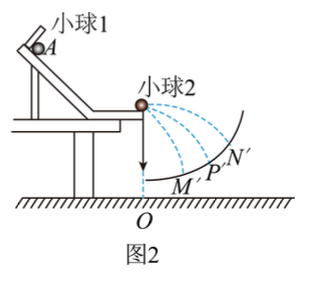
\includegraphics[width=0.3\textwidth,keepaspectratio]{./pictures/1.2-4.png}

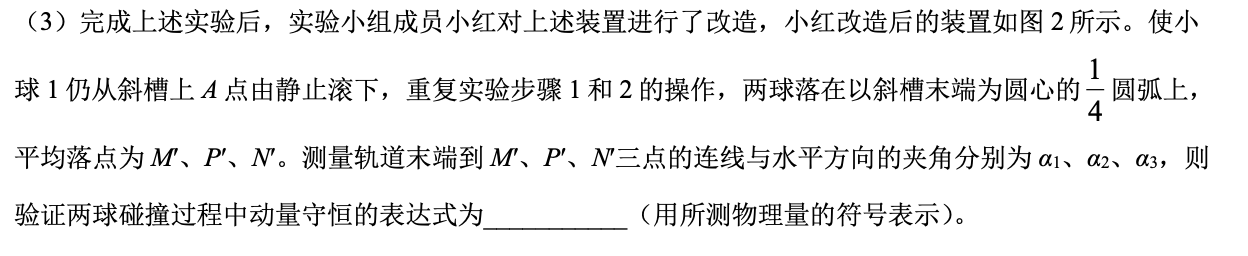
\includegraphics[width=0.95\textwidth,keepaspectratio]{./pictures/1.2-5.png}

\begin{itemize}
    \item 总结:夹角$\alpha$为位移偏转角.这类题目已知位移偏转角同时还有几何约束那么易得
          $$
              \begin{cases}
                  x = R \cos{\alpha} = v_{x} t             \\
                  y = R \sin{\alpha} = \frac{1}{2} g t^{2} \\
              \end{cases}
          $$

          $$
              \lra v_{x} = \sqrt{\frac{gR}{2}} \vdot \sqrt{\frac{\cos^{2}{\alpha}}{\sin{\alpha}}} \quad  \llra \quad  v_{x}  \propto  \sqrt{\frac{\cos^{2}{\alpha}}{\sin{\alpha}}}
          $$

\end{itemize}

\vspace{2em}

\subsubsection{IV-2:平抛-圆弧约束的最值问题}
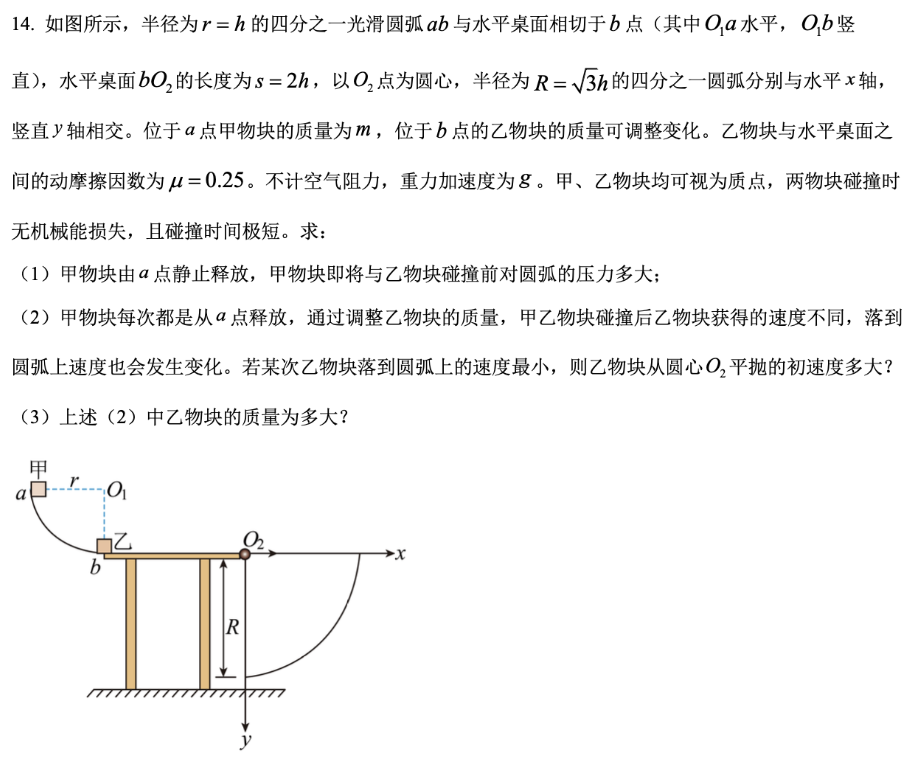
\includegraphics[width=0.45\textwidth,keepaspectratio]{./pictures/1.2-6.png}

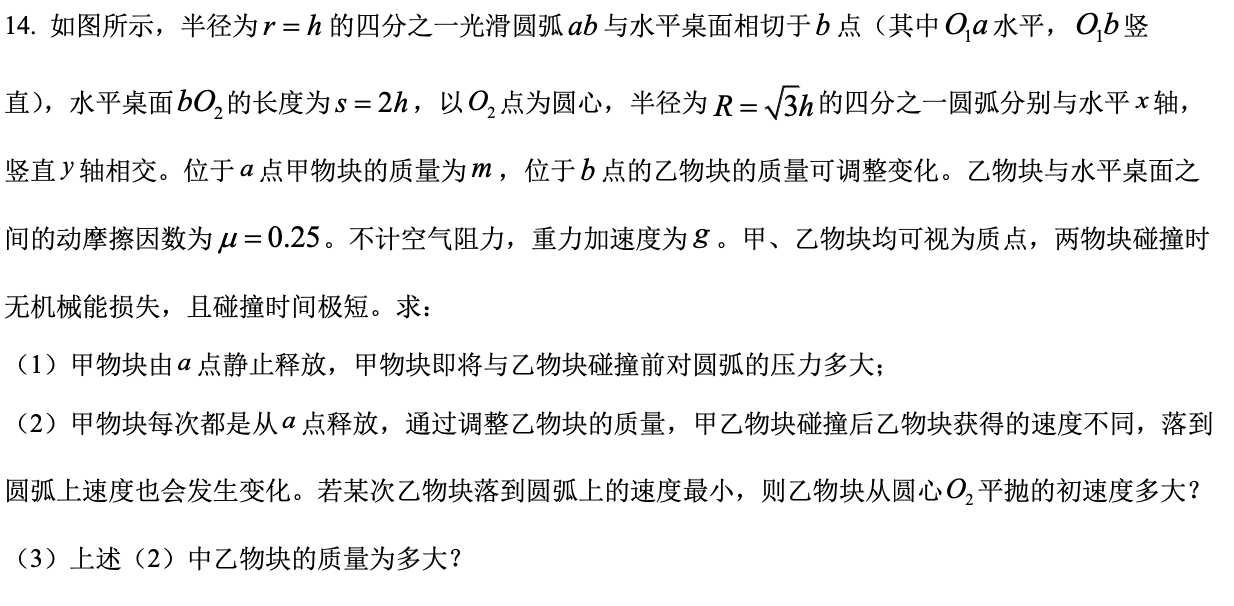
\includegraphics[width=0.95\textwidth,keepaspectratio]{./pictures/1.2-7.png}

\begin{itemize}
    \item 总结:\quad 在解方程组的时候,选择去消掉$t$直接得到$v = f(v_{0})$是非常困难的,事实上先解出$v = f(y)$求得最小的
          $y_{min}$,那么就可得到最小的$v_{ymin}$进而得到最小的$v = \sqrt{gh}$
\end{itemize}

\vspace{2em}


\subsection{2022-2023巴蜀中学下学期期末}
\subsubsection{I-13:电路中的变化量分析}
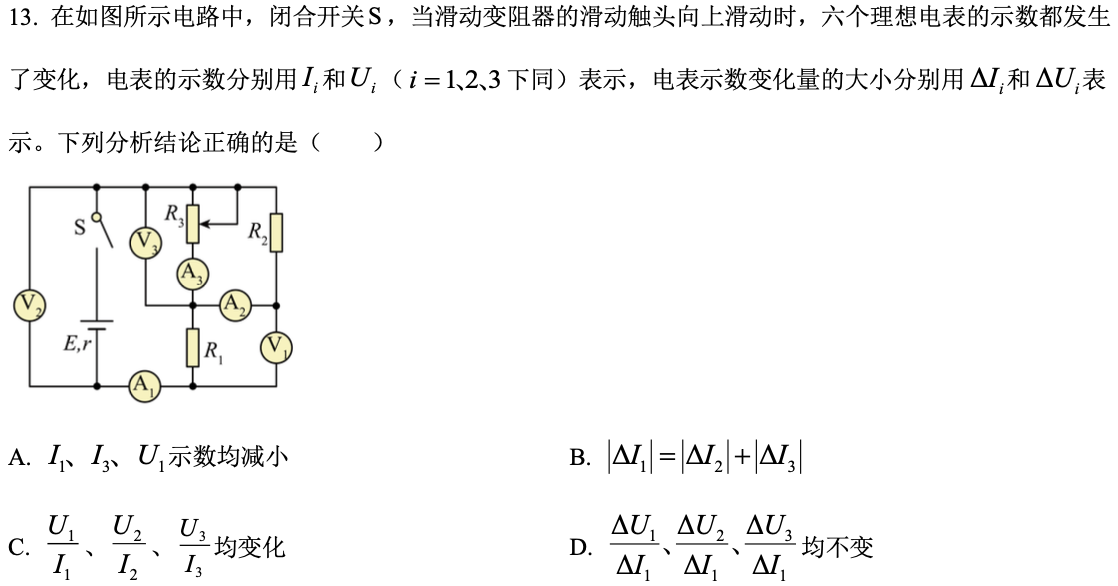
\includegraphics[width=0.95\textwidth,keepaspectratio]{./pictures/1.3-2.png}

\begin{itemize}
    \item 总结: \quad 最好写出回路的表达式$E = U_{2} + I_{1}r  \quad U_{3} = E - I_{1}(R_{1} + r)$
\end{itemize}

\vspace{2em}

\subsubsection{II-2:电路的测量误差}
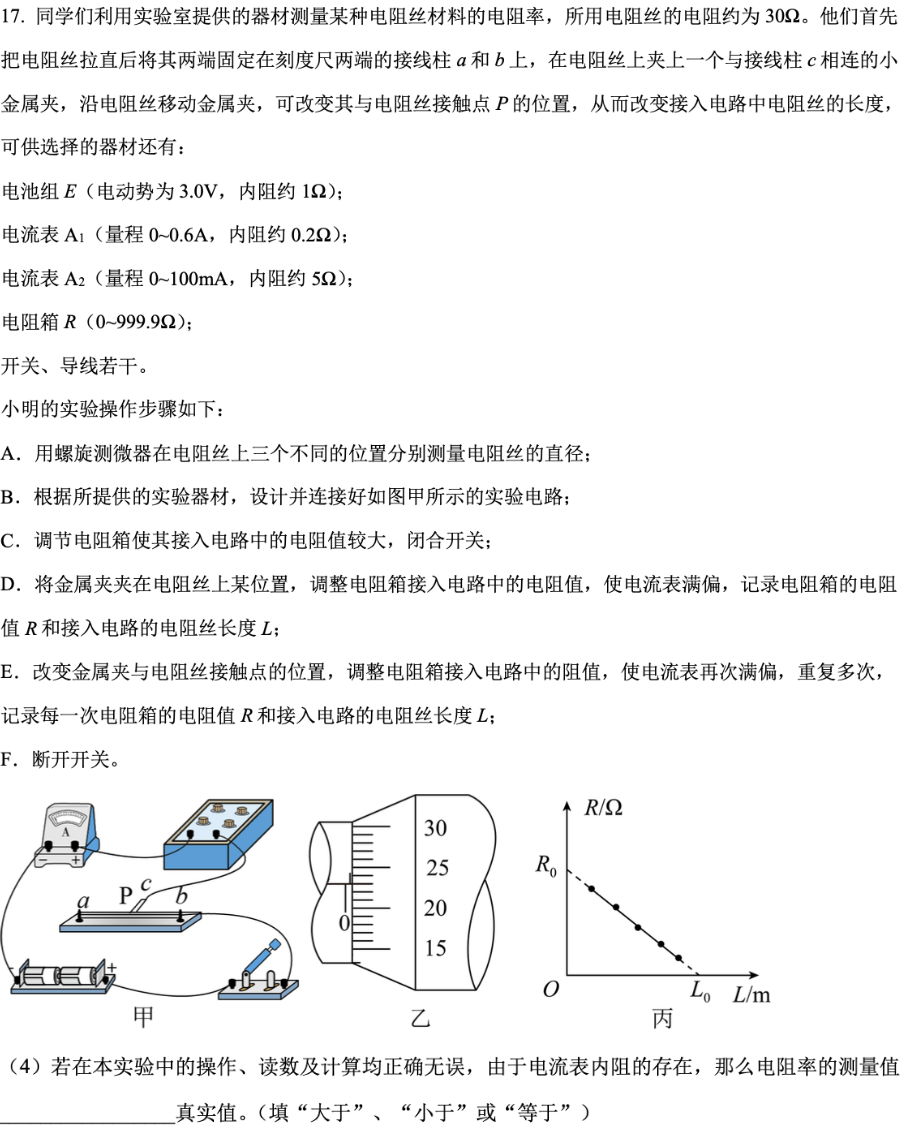
\includegraphics[width=0.95\textwidth,keepaspectratio]{./pictures/1.3-3.png}

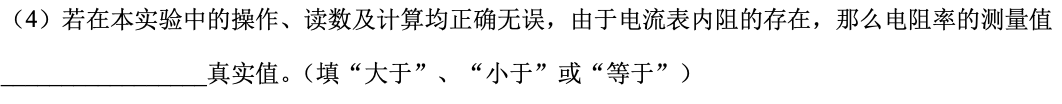
\includegraphics[width=0.95\textwidth,keepaspectratio]{./pictures/1.3-4.png}

\begin{itemize}
    \item 总结:\quad 官解结果正确但是思路奇怪,$R_{0}$会发生变化,存在电流表内阻时
          $$
              R_{0} = \frac{E}{I} - r
          $$
          所以$R_{0}$测量值偏小,但事实上实验步骤并不直接得到$R_{0}$,而是通过延长线的方式,因此$L_{0}$并非不变化的

          $$
              R_{i} = \frac{E}{I_{满偏}} - r -\frac{4\rho}{\pi d^{2}} L_{i}
          $$

          实验的测量值是准确的,因此忽略电流表内阻与仅仅是将直线向下移动,并不影响斜率,所以结果是等于
\end{itemize}

\vspace{2em}

\subsection{2022-2023南开中学高一下期末}
\subsubsection{I-6:光的几何表示问题}
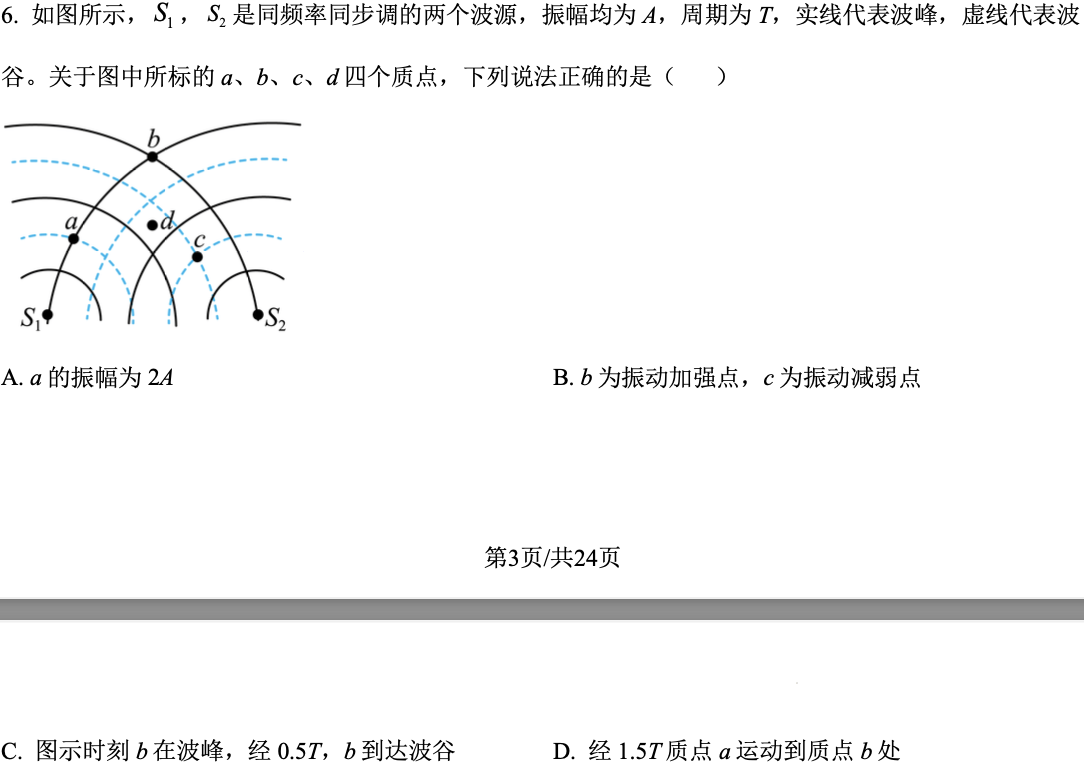
\includegraphics[width=0.95\textwidth,keepaspectratio]{./pictures/1.4-1.png}

\begin{itemize}
    \item 正解:\quad C
    \item 总结:\quad 此为光波的另一种表现方式,同时\textbf{振动加强点包括波峰叠加和波谷叠加},D选项,质点$a$实际仅在平衡位置振动,并不产生其它方向的位移
\end{itemize}

\vspace{2em}


\subsubsection{I-8:单摆+受迫振动}
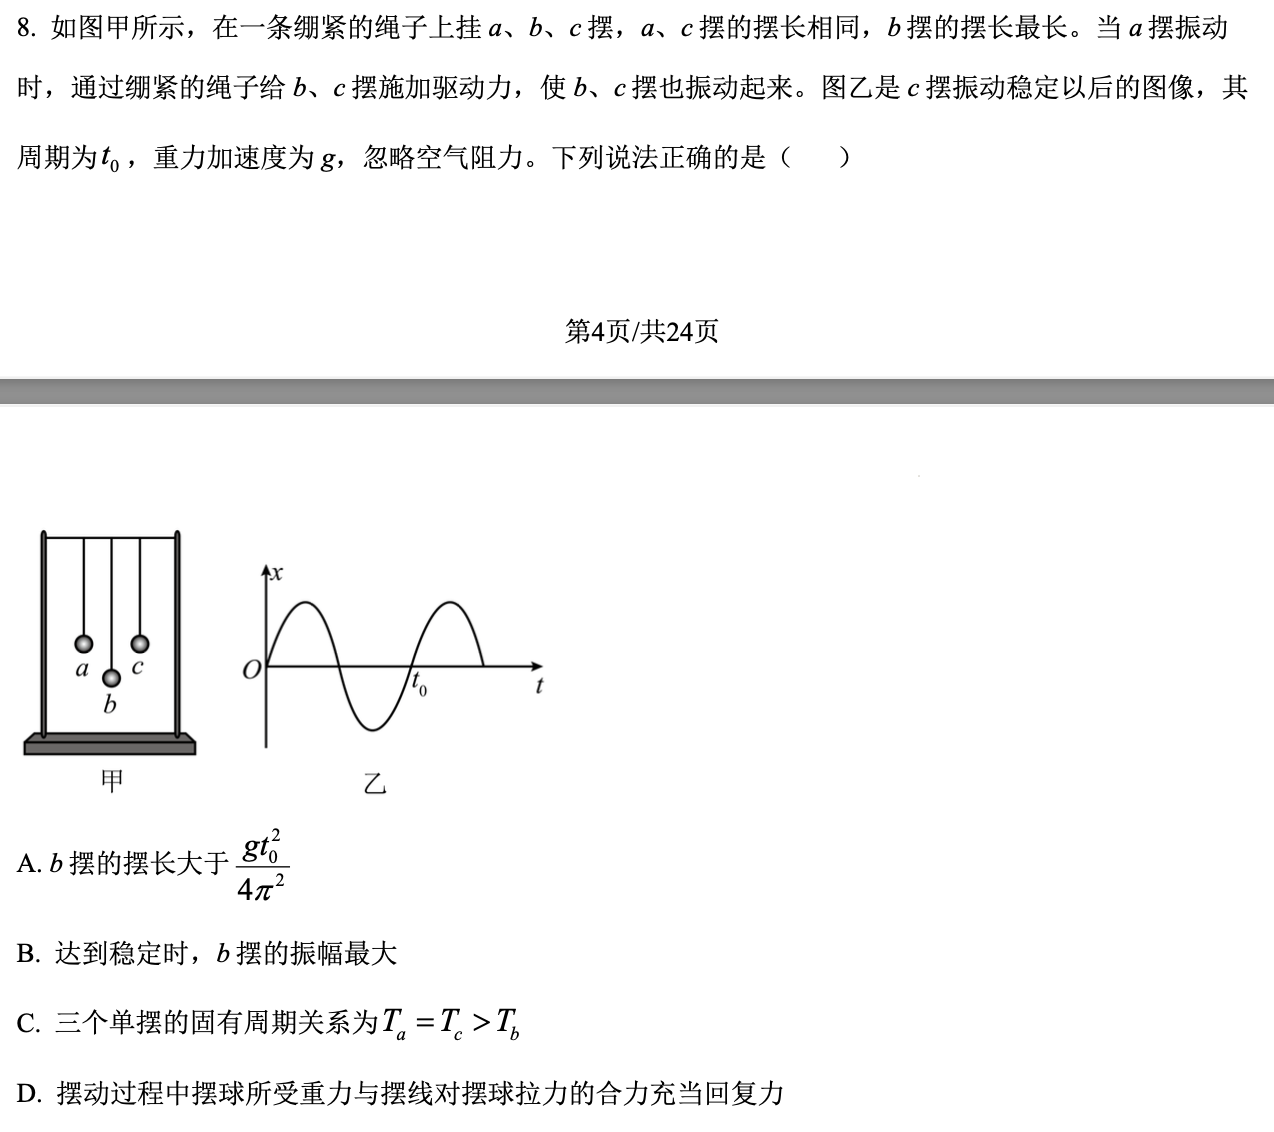
\includegraphics[width=0.95\textwidth,keepaspectratio]{./pictures/1.4-2.png}

\begin{itemize}
    \item 正解:\quad A
    \item 总结:\quad 单摆周期公式死记硬背,受迫振动:在周期性外力的持续作用下而进行的振动称为\textbf{受迫振动},振动稳定后齐\textbf{频率}等于外力驱动频率
          $$
              T = 2 \pi \sqrt{\frac{L}{g}}
          $$

          \begin{itemize}
              \item[]
                  \begin{proof}
                      证明运动为简谐运动,仅需证明回复力$F = -kx$(多次进行小量近似,很简单)\\
                  \end{proof}
              \item[]
                  \begin{proof}
                      证明简谐运动的周期(更复杂的方法请参考朗道等高阶解法)
                      \begin{align*}
                          F = -\frac{mg}{L} \vdot x                                               & = m \dv[2]{x}{t}           \\
                          \dv[2]{x}{t} + \frac{g}{L}x                                             & = 0                        \\
                          \text{令} \quad \omega                                                   & = \sqrt{\frac{g}{L}}       \\
                          \dv[2]{x}{t} + \omega^{2}x                                              & = 0                        \\
                          \text{特征根方程} \quad r^{2} = \omega^{2} \quad r                           & = \pm \omega i             \\
                          x = C \sin{(\omega t + \phi)} \quad \lra \quad T = \frac{2 \pi}{\omega} & = 2 \pi \sqrt{\frac{L}{g}}
                      \end{align*}
                  \end{proof}
          \end{itemize}
\end{itemize}

\begin{figure}[h]
    \centering
    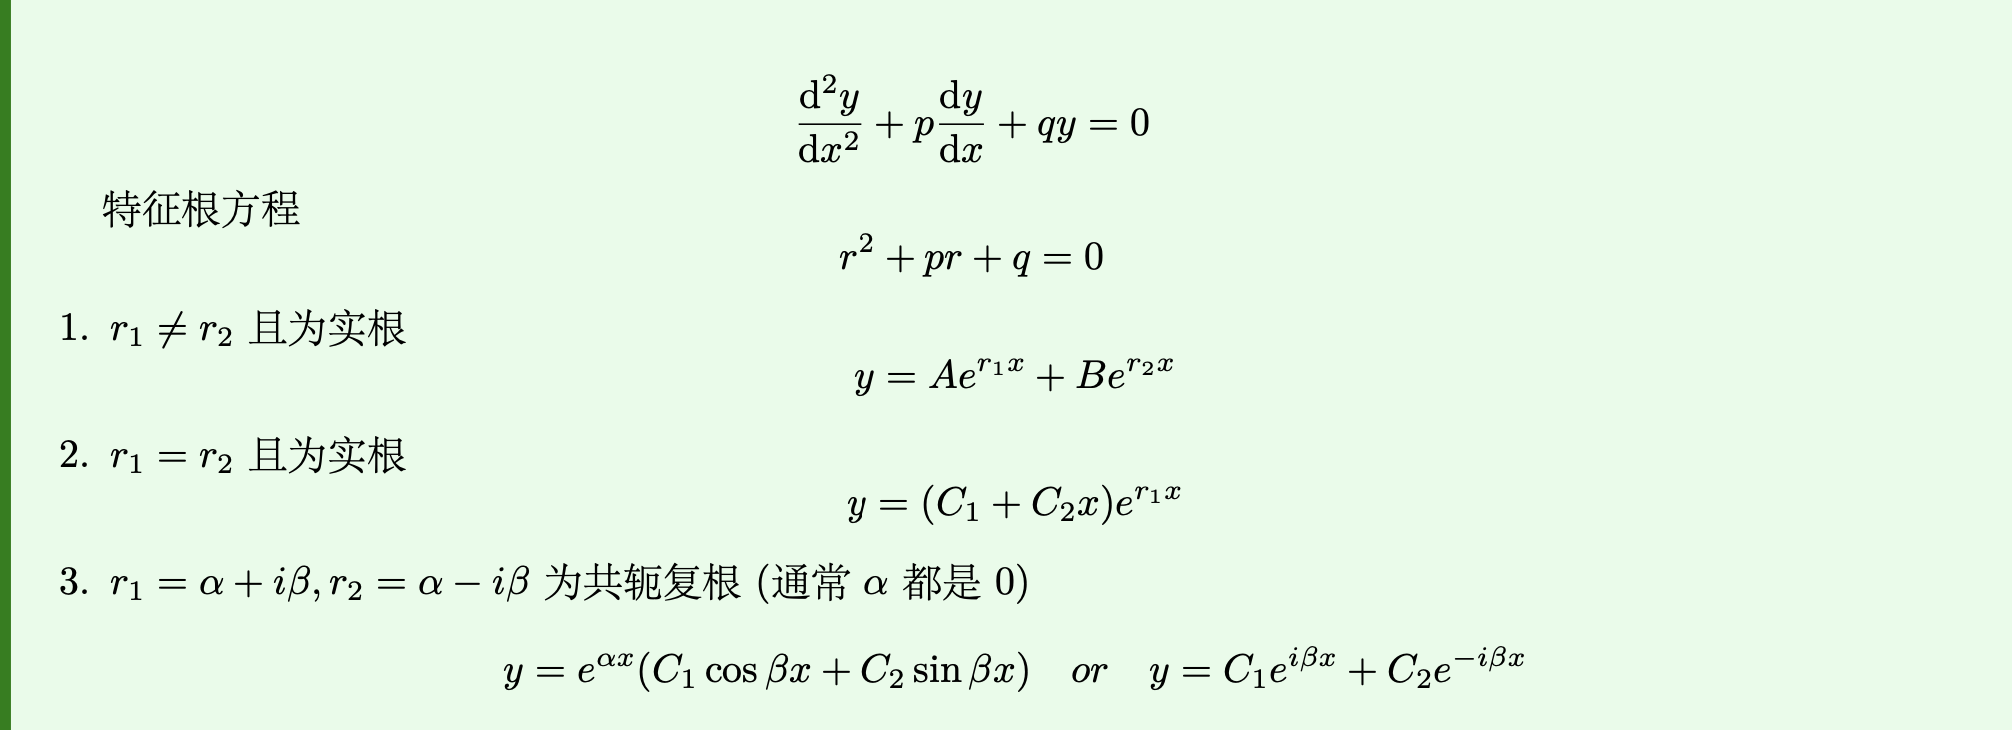
\includegraphics[width=\textwidth,keepaspectratio]{./pictures/1.4-3.png}
\end{figure}

\vspace{2em}

\subsubsection{I-10:折射率问题}
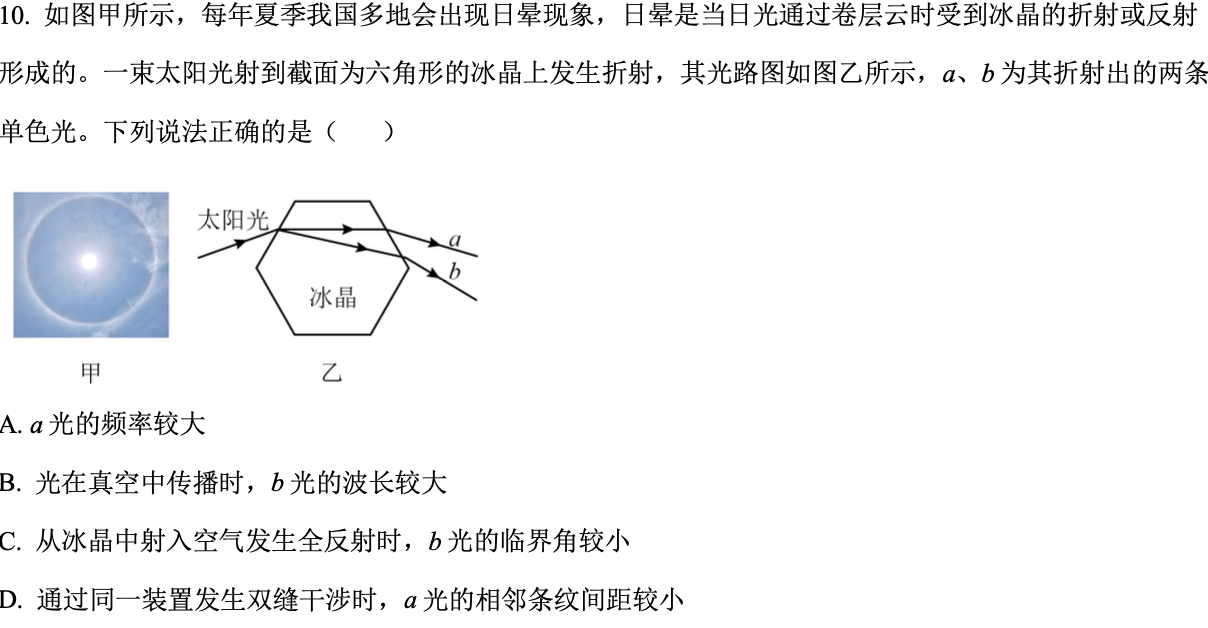
\includegraphics[width=0.95\textwidth,keepaspectratio]{./pictures/1.4-4.png}

\begin{itemize}
    \item 正解:\quad C
    \item 总结:\quad
          \begin{itemize}
              \item 光的\textbf{频率}$\nu$是本质属性,在任何介质下传播都不发生改变
              \item 同一介质中不同频率的光,\textbf{其折射率随频率单调递增}
              \item 同一光在不同介质的折射率不同
          \end{itemize}
    \item 扩展:\quad
          \begin{formal}
              符号说明

              \begin{tabular}{|c|c|c|c|c|c|c|c|c|c|}
                  \hline
                  频率  & 折射率 & 速度  & 临界角 & 波长        & 动量  & 干涉            & 能量            & 逸出功     & 逃逸光子动能  \\
                  \hline
                  $f$ & $n$ & $v$ & $C$ & $\lambda$ & $p$ & $\triangle x$ & $\varepsilon$ & $w_{0}$ & $E_{k}$ \\
                  \hline
              \end{tabular}

              \vspace*{2em}

              \begin{itemize}
                  \item 同一介质中不同频率的光

                        \vspace*{1em}
                        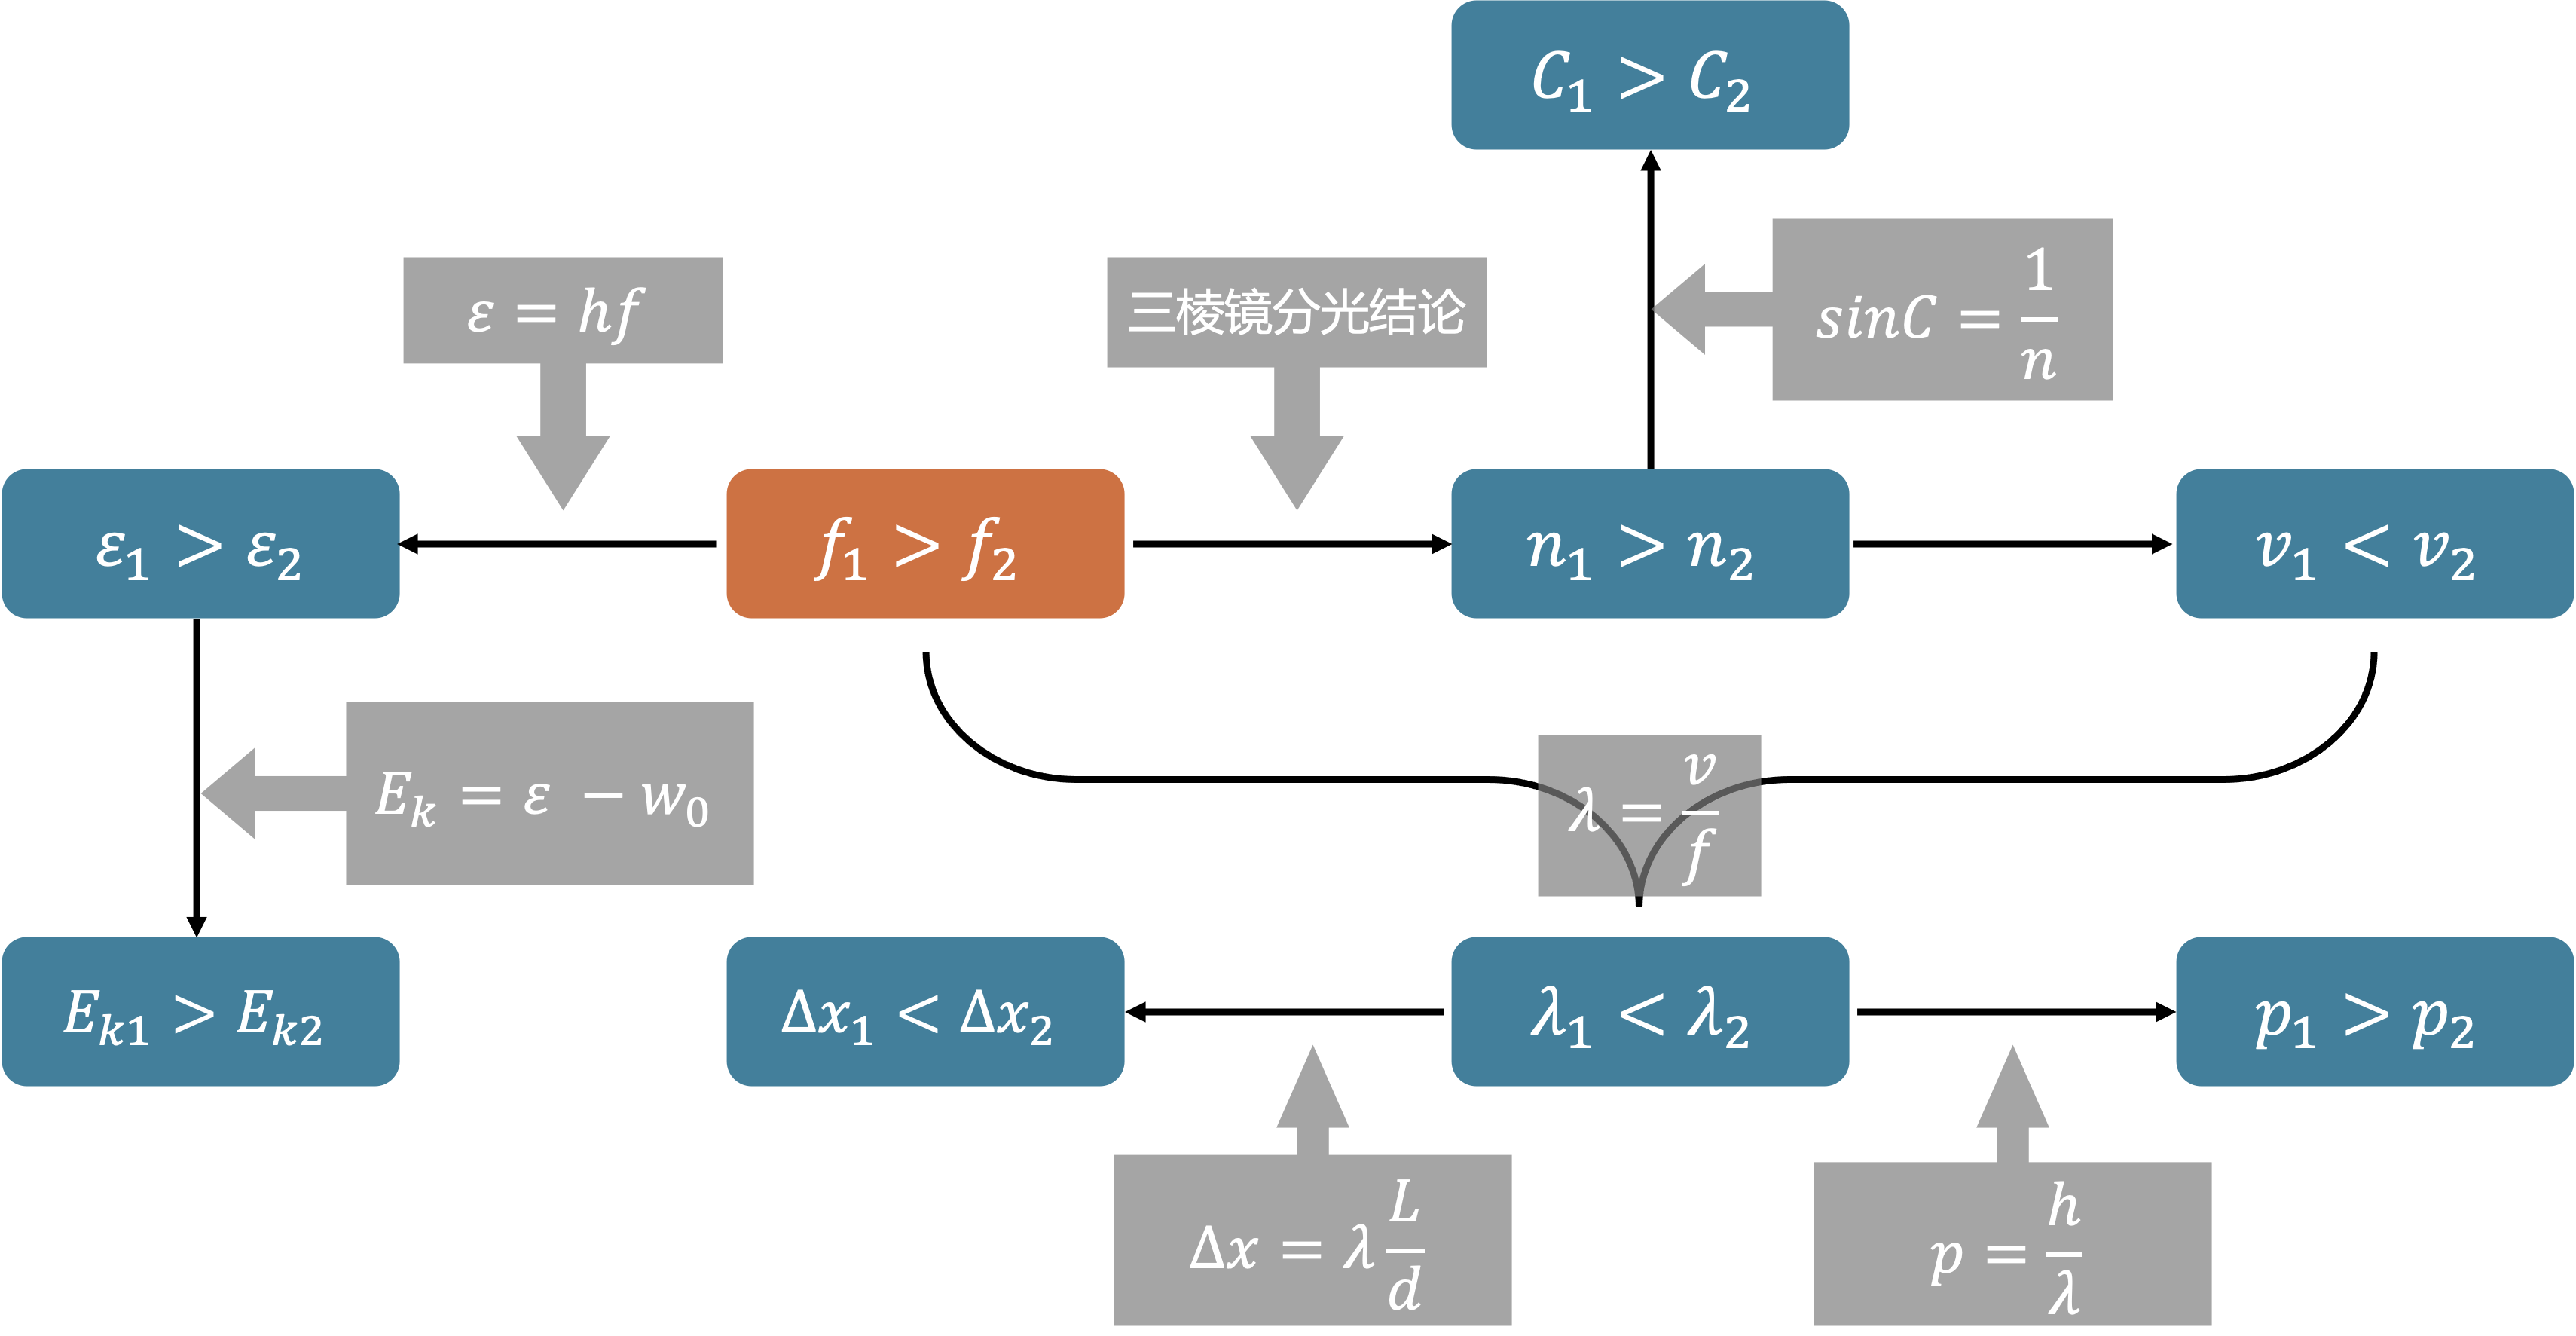
\includegraphics[width=40em,keepaspectratio]{./pictures/1.4-5.png}

                        \vspace*{2em}

                  \item 同一频率的光在不同介质(下标表示不同介质中)中

                        \vspace*{1em}
                        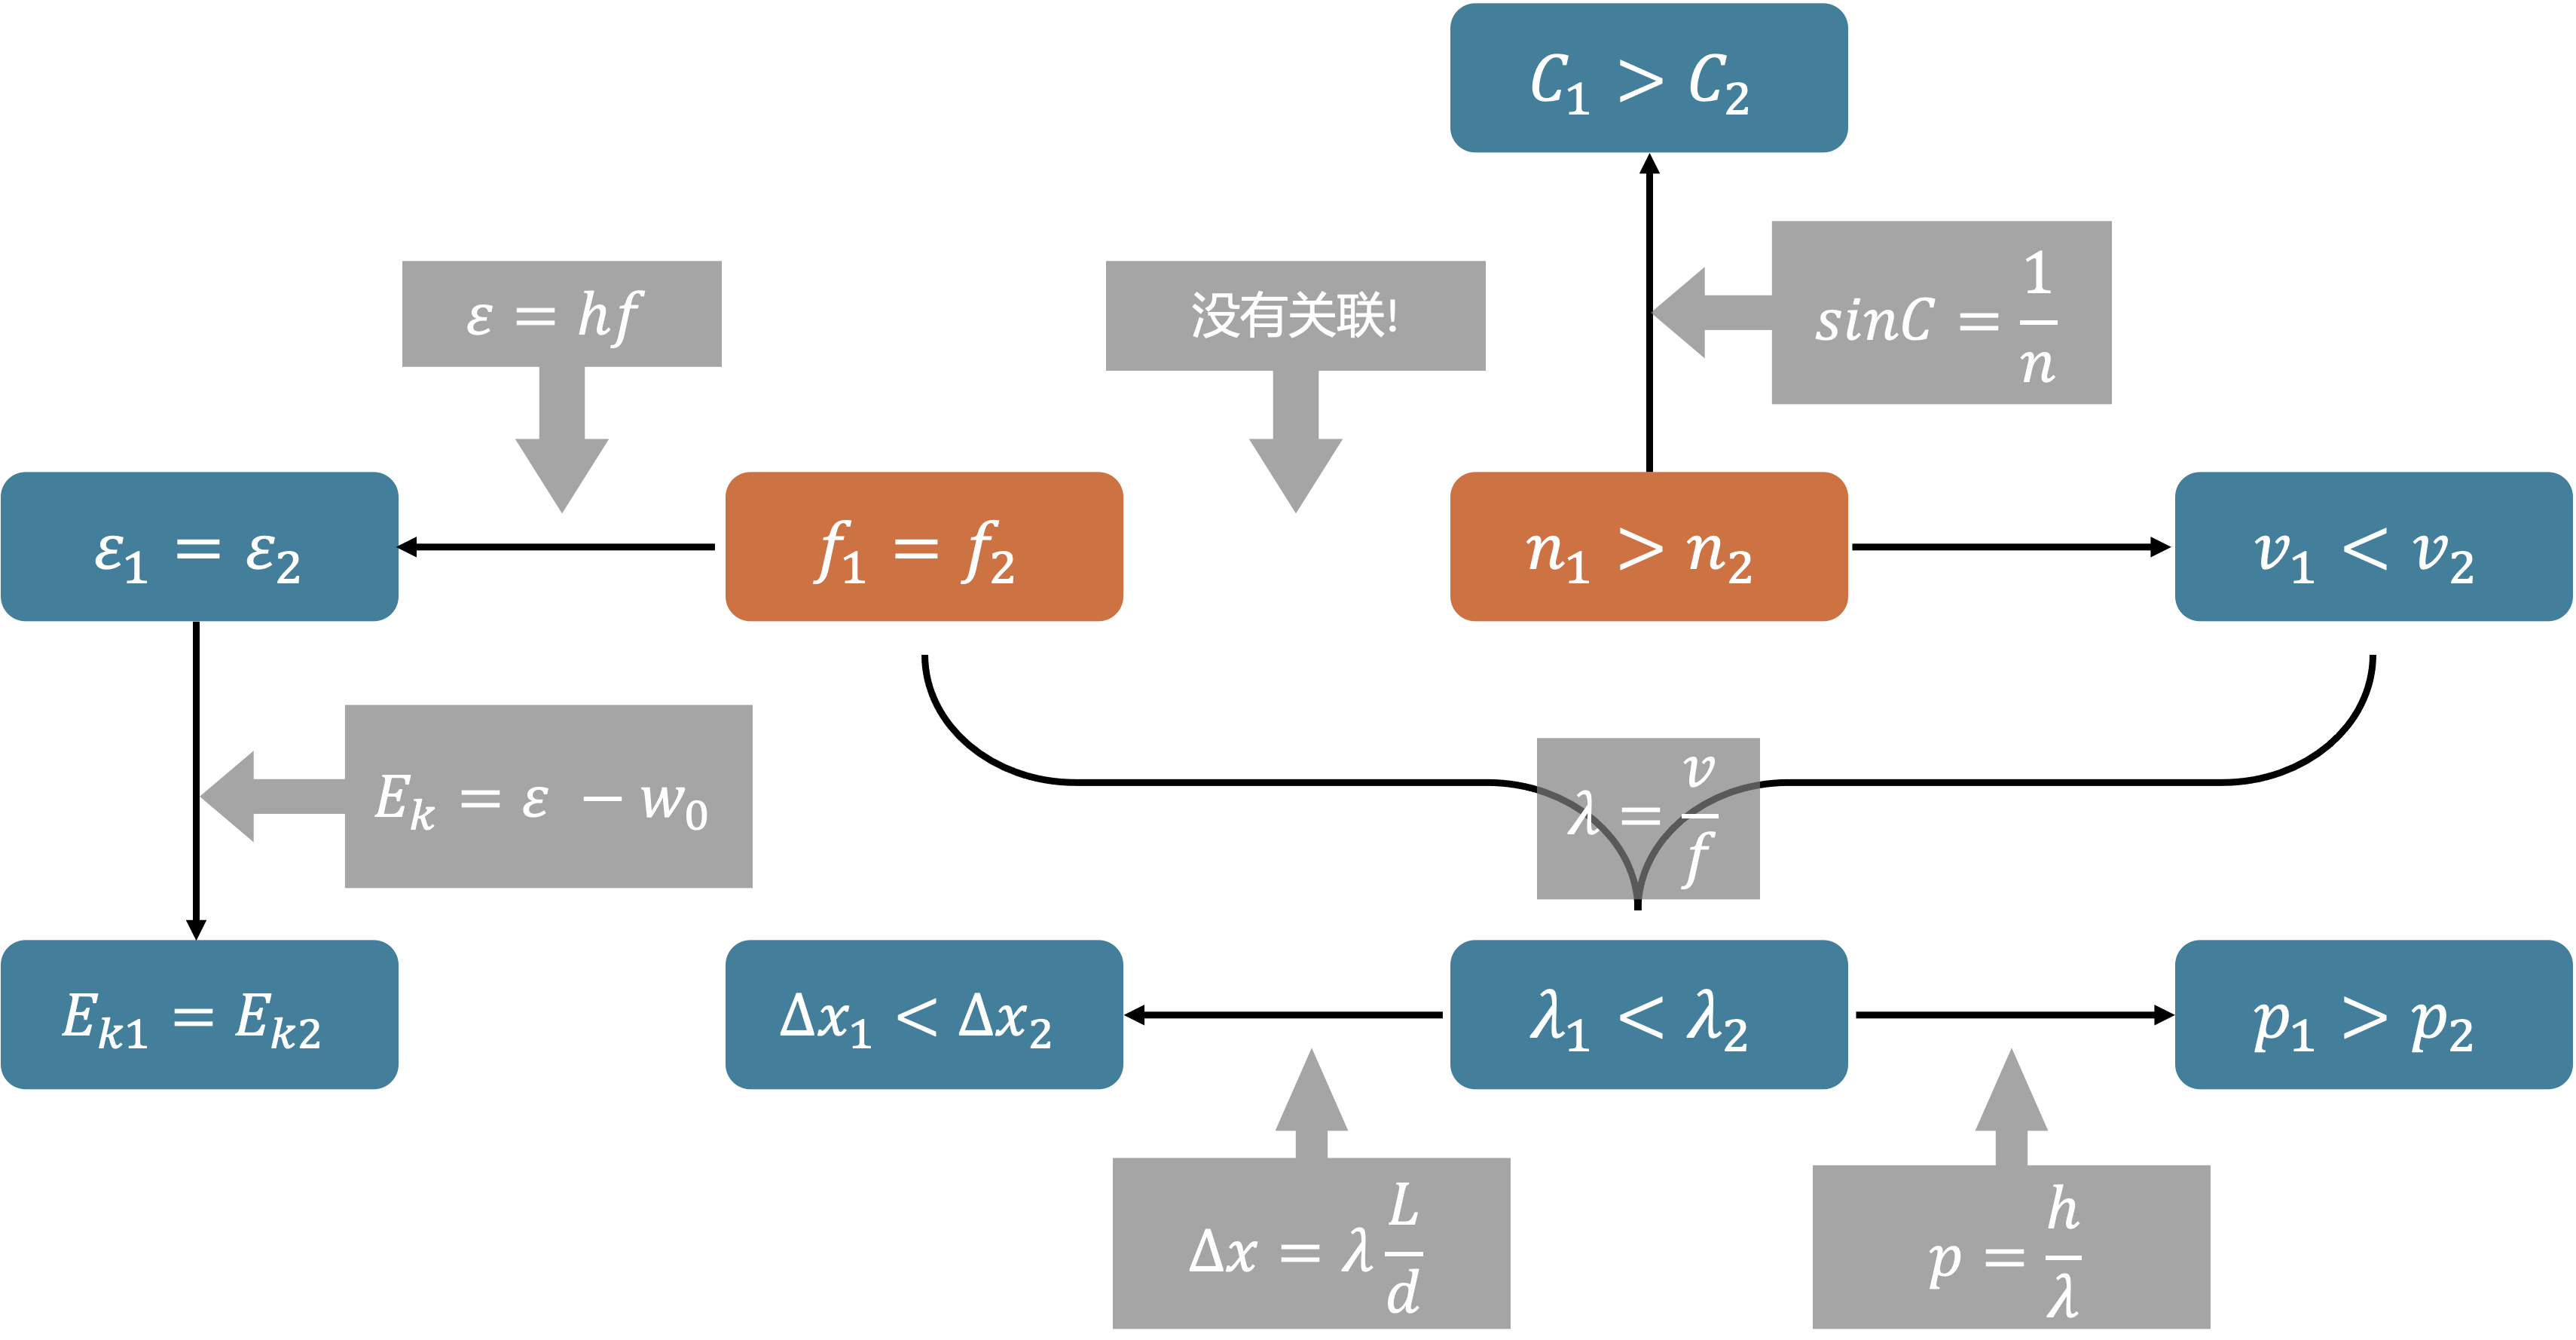
\includegraphics[width=40em,keepaspectratio]{./pictures/1.4-6.png}
              \end{itemize}
          \end{formal}
\end{itemize}

\vspace{2em}

\subsection{2022-2023育才中学期末模拟题(六)}
\subsubsection{II-3:水平初动量不为0的杆相互作用模型}

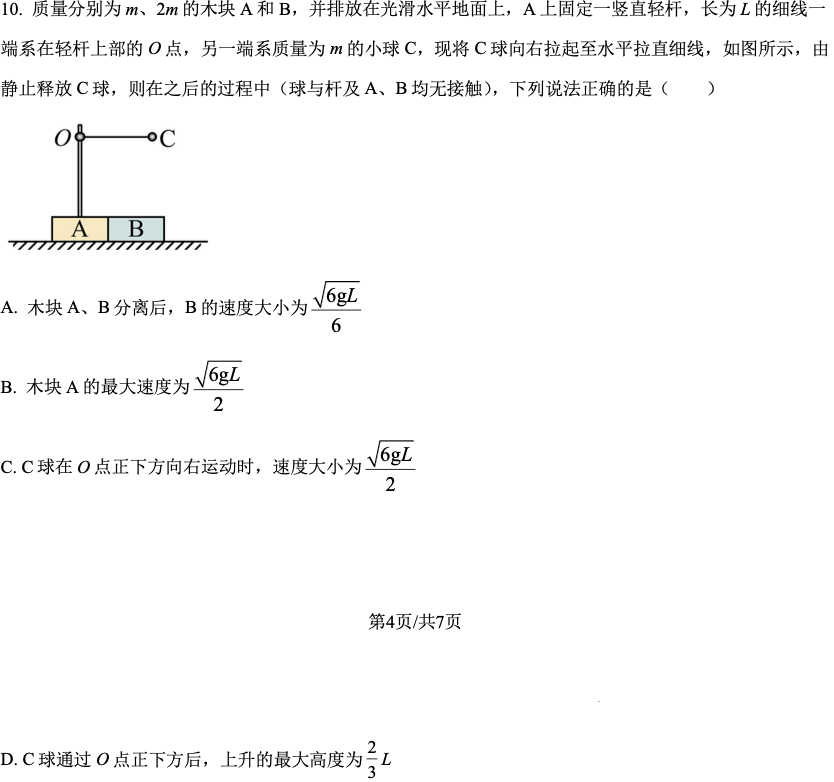
\includegraphics[width=0.95\textwidth,keepaspectratio]{./pictures/1.5-1.png}

\begin{itemize}
    \item 正解:\quad ABD
    \item 总结:\quad 是一类通过杆相互作用的水平动量守恒模型,但是注意系统初动量不为0
\end{itemize}

\vspace{2em}

\subsection{2022-2023育才中学期末模拟题(三)}
\subsubsection{I-6:调和定律-新颖题目}

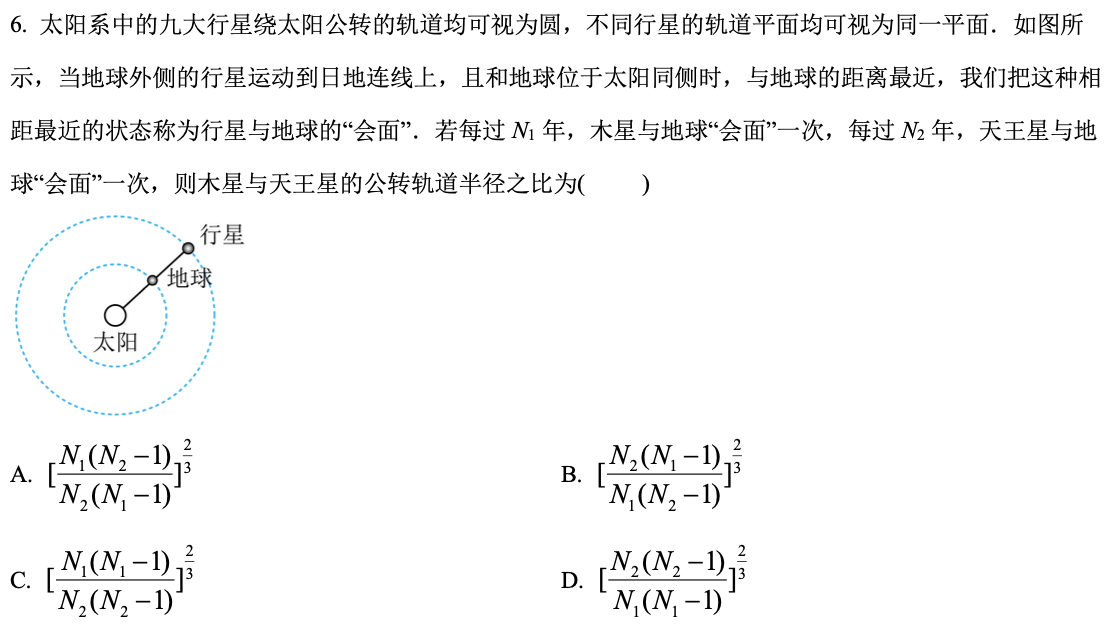
\includegraphics[width=0.95\textwidth,keepaspectratio]{./pictures/1.5-2.png}

\begin{itemize}
    \item 正解:\quad A
    \item 总结:\quad 注意理解一年的意义
\end{itemize}

\subsubsection{II-3:连续弹碰(牛顿摆)}

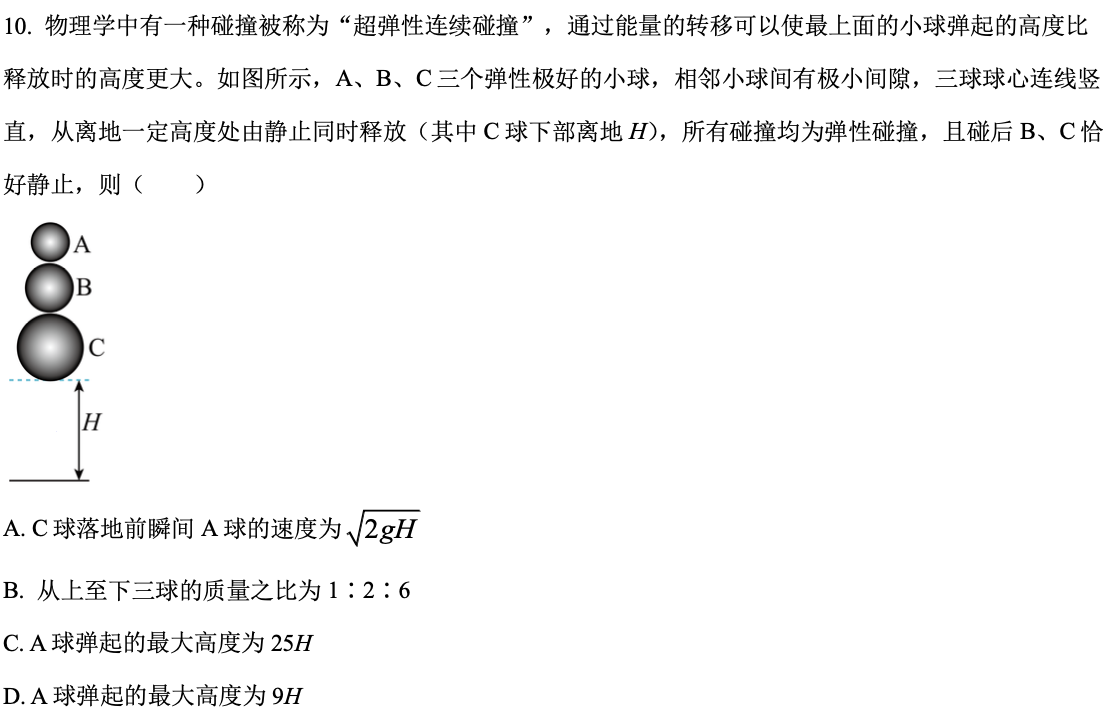
\includegraphics[width=0.95\textwidth,keepaspectratio]{./pictures/1.5-3.png}

\begin{itemize}
    \item 正解:\quad ABD
    \item 总结:\quad 逐个分析即可
    \item 扩展:\quad 牛顿摆的分析方法也是先研究瞬时碰撞的两个物体,并进行传递
\end{itemize}

\vspace{2em}

\subsection{2022-2023一中高一下期末}
\subsubsection{III-1:折射率实验}

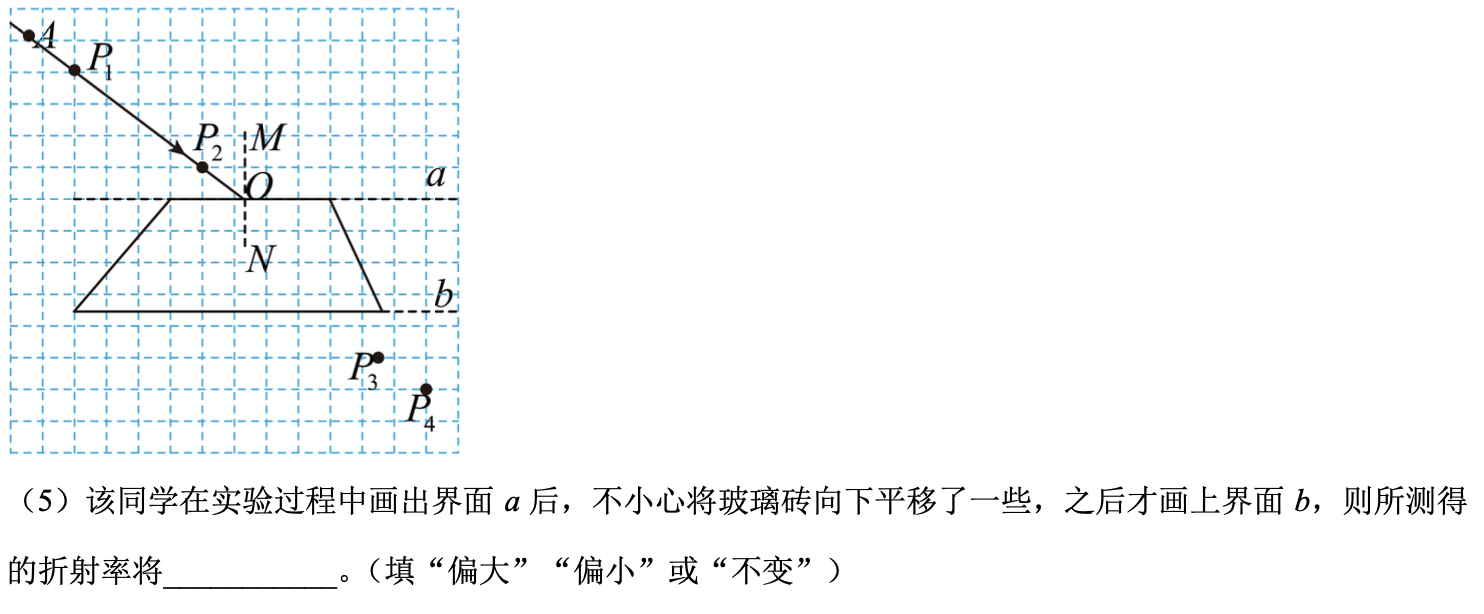
\includegraphics[width=0.95\textwidth,keepaspectratio]{./pictures/1.6-1.png}

\begin{itemize}
    \item 正解:\quad 偏小
    \item 总结:\quad 玻璃砖整体平移,非平行玻璃砖的测量是准确的;
          其他情况$d_{\text{画}}$\,$d_{\text{玻}}$的大小关系与$n_{\text{测}}$\,$n_{\text{真}}$相反    \\
          此题中由于将玻璃下移后才画上下边界,因此$d_{\text{画}} > d_{\text{真}} \quad \lra \quad n_{\text{测}} < n_{\text{真}}$
\end{itemize}


\vspace{2em}


\section{高二}

\subsection{机械振动专题}
\subsubsection{I-1:起振方向未知的多解问题}
一个弹簧振子沿$x$做简谐运动,平衡位置在坐标原点,振幅为$0.2m$.$t= 0$时振子的位移为$-0.1m$,$t = 0.5s$时位移第一次为$0.1m$,则振子的周期可能是
$$
    A. 1s   \hspace{10em}    B. 1.5s      \hspace{10em}    C. 2s      \hspace{10em}    D. 3s
$$

\begin{itemize}
    \item 正解:\quad AD
    \item 总结:\quad 起振方向未知,存在多解
          \begin{align*}
              y & = 0.2\sin{(\omega t + \varphi)}                            \\
              t & = 0  \quad  \sin{\varphi} = -\dfrac{1}{2} \quad \lra \quad
              \begin{cases}
                  \varphi = - \dfrac{\pi}{6} \\
                  \,                         \\
                  \varphi = - \dfrac{5\pi}{6}
              \end{cases}                                     \\
              t & = 0.5s \quad \sin{0.5 \omega  + \varphi } = \dfrac{1}{2}   \\
                & \begin{cases}
                      \dfrac{\omega}{2} - \dfrac{\pi}{6} = \dfrac{\pi}{6} \\
                      \,                                                  \\
                      \dfrac{\omega}{2} - \dfrac{5\pi}{6} = \dfrac{\pi}{6}
                  \end{cases}
              \quad \lra  \quad
              \begin{cases}
                  \omega = \dfrac{2\pi}{3} \quad \lra \quad T = \dfrac{2\pi}{\omega} = 3s \\
                  \,                                                                      \\
                  \omega = 2\pi \quad \lra \quad T = \dfrac{2\pi}{\omega} = 1s
              \end{cases}
          \end{align*}

    \item 扩展:\quad

          造成波的多解性的三大原因:
          \begin{itemize}
              \item \textbf{波的周期性:}\hspace{1em}
                    $\begin{cases}
                            \text{时间周期性:时间间隔}\triangle t \text{与周期} T \text{的关系不明确} \\
                            \text{空间周期性:波传播距离}\triangle x \text{与波长} \lambda \text{的关系不明确}
                        \end{cases}$

              \item \textbf{波的双向性:}\hspace{1em}
                    $\begin{cases}
                            \text{传播方向双向性:波的传播方向不确定} \\
                            \text{振动方向双向性:质点振动方向不确定}
                        \end{cases}$

              \item \textbf{波形隐含性:}\hspace{1em}
                    $\begin{cases}
                            \text{在波动问题中,有时只给出几个特殊点} \\
                            \text{(大多是两个特殊的点)的运动状态,其余信息均处于隐含状态}
                        \end{cases}$
          \end{itemize}

\end{itemize}

\vspace{2em}

\subsubsection{I-2:球面波干涉图像问题}
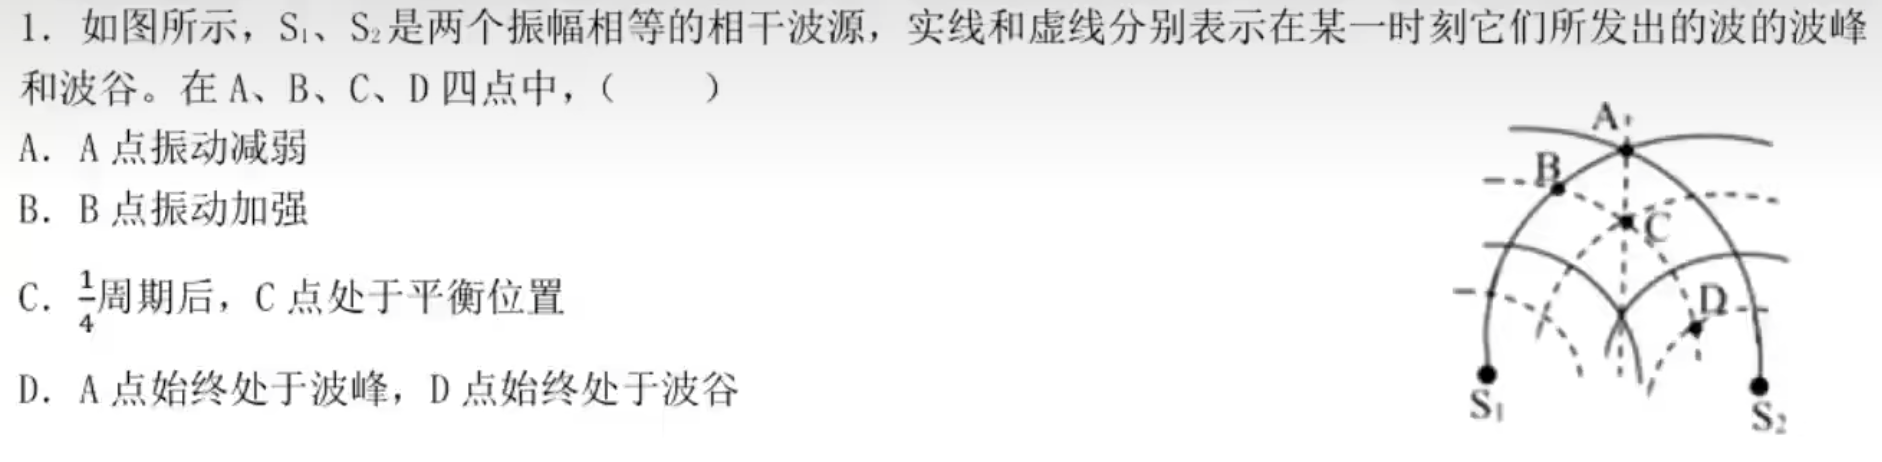
\includegraphics[width = 0.95\textwidth]{./pictures/2.1-1.png}

\begin{itemize}
    \item 正解:\quad C
    \item 总结:\quad C选项,c点为振动加强点,仅仅是振幅变大,并非不在平衡位置振动,研究$\frac{1}{T}$时间后
          的位置情况,是根据叠加波(周期不变)的传播来看,经过该时间后,波谷达到平衡位置,所以C选项正确
    \item 扩展:\quad 此类干涉图的所有振动加强点的连线是双曲线.有的此类图形未必是干涉图像,比如两个水波的叠各自具有不同的周期,因此某个点振动加强或减弱并非恒定
\end{itemize}

\begin{center}
    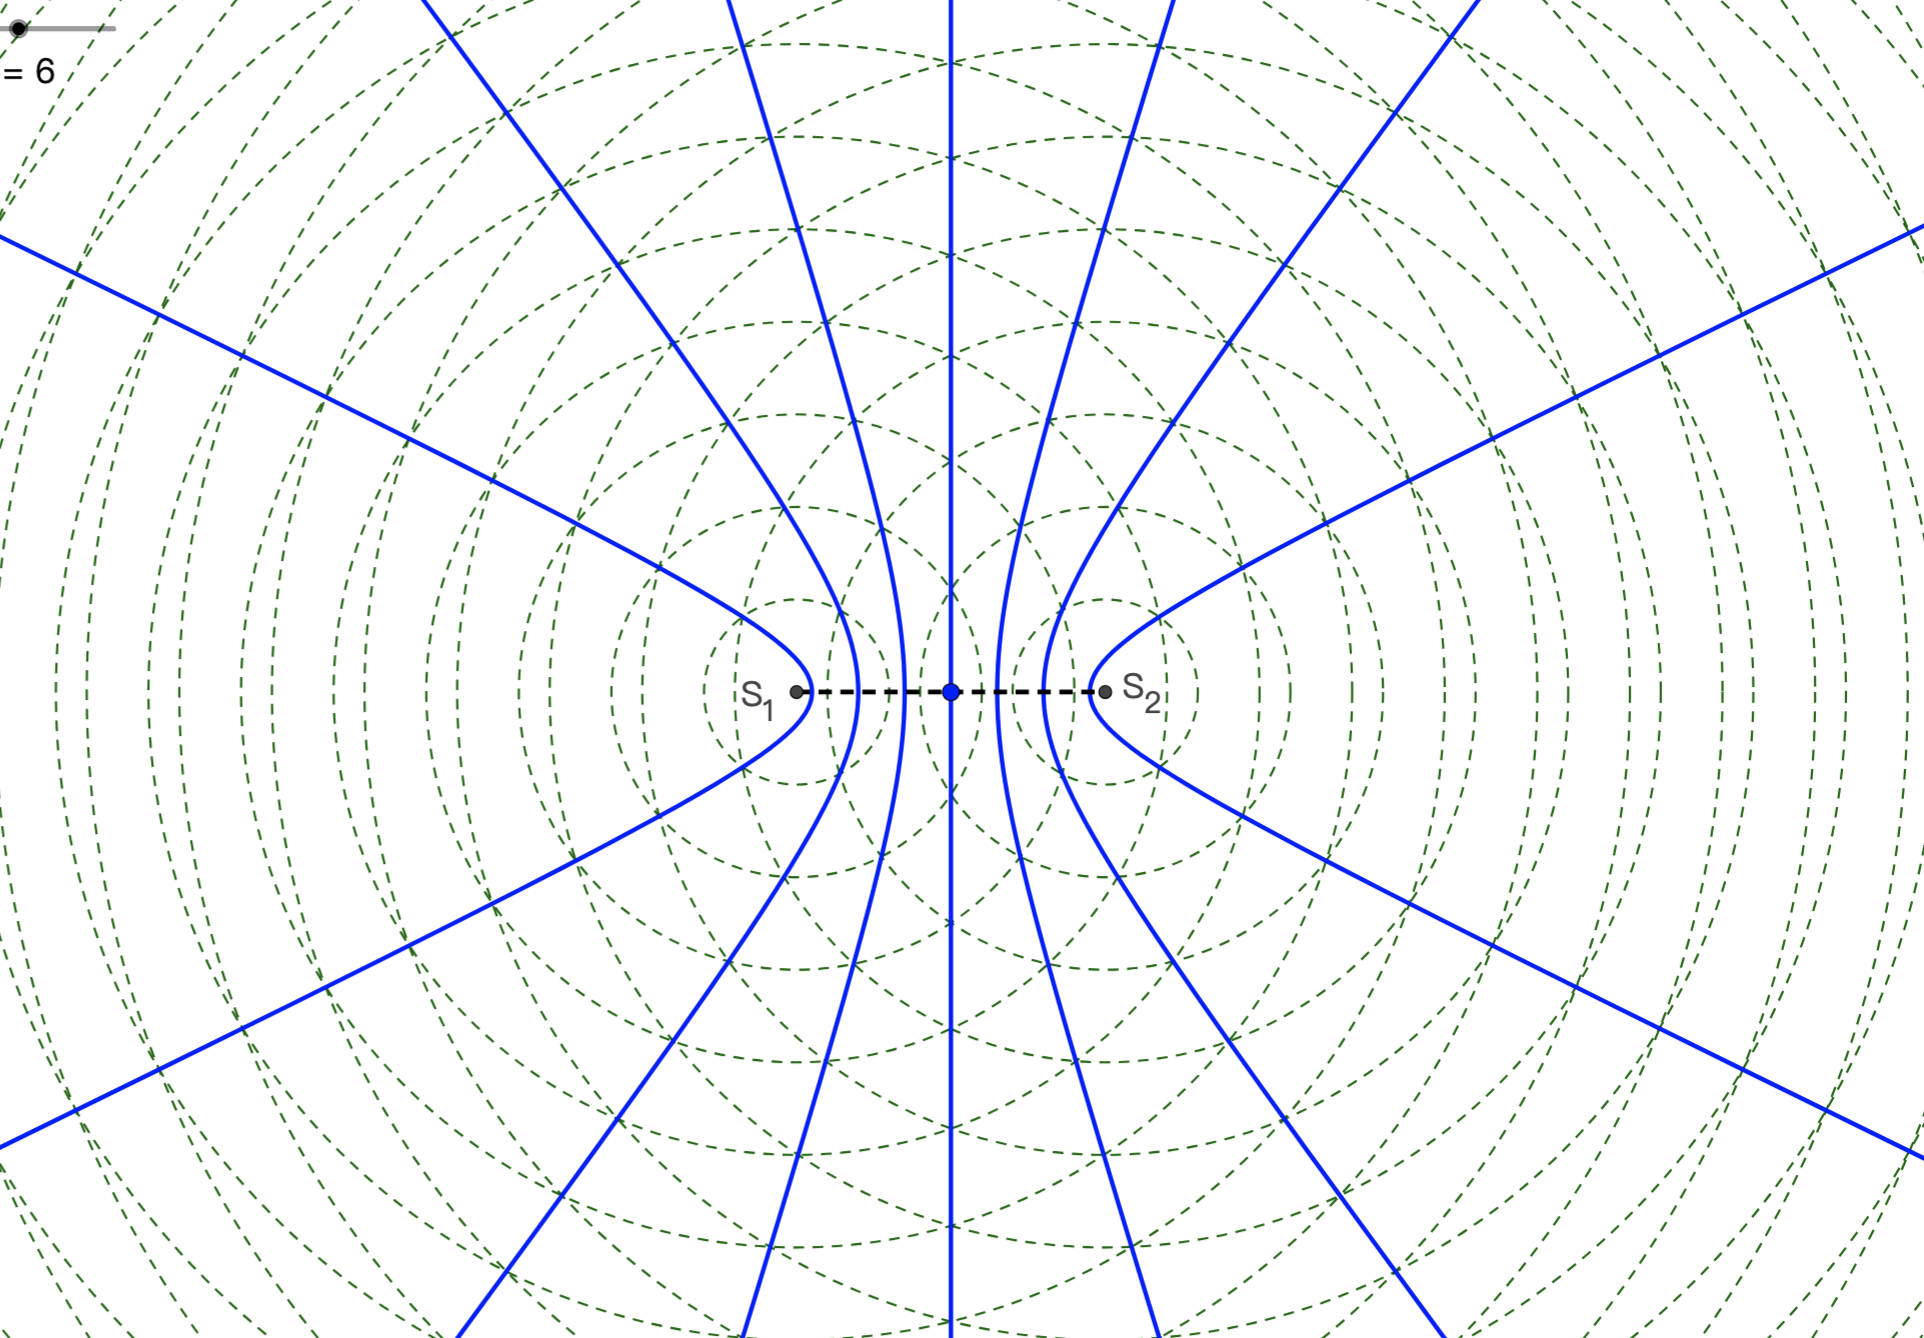
\includegraphics[width = 0.6\textwidth]{./pictures/2.1-2.png}
\end{center}

\vspace{2em}

\subsubsection{I-3:球面波非干涉图像问题}
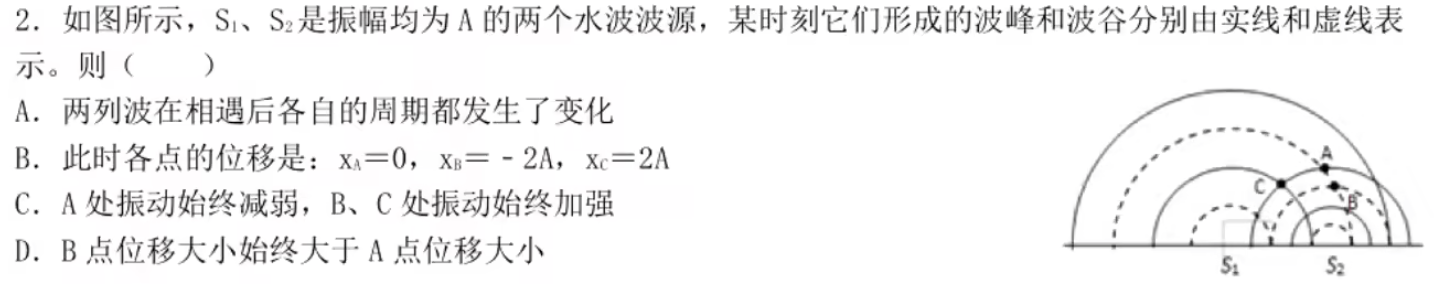
\includegraphics[width = 0.95\textwidth]{./pictures/2.1-6.png}

\begin{itemize}
    \item 正解:\quad B
    \item 总结:\quad 两个水波没有特定说明则是非相干波源,因此振幅的加强或减弱是非恒定的
\end{itemize}

\vspace{2em}

\subsubsection{I-4:折射率几何求解}
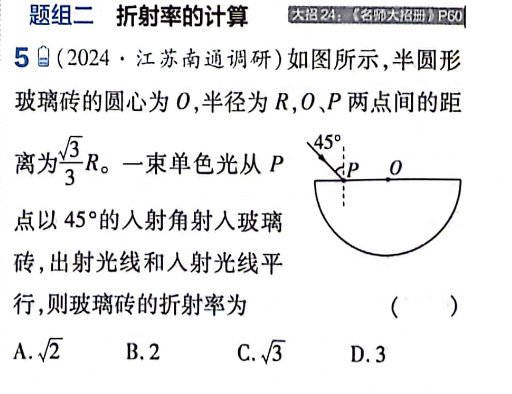
\includegraphics[width = 25em]{./pictures/2.1-9.png}

\begin{itemize}
    \item 正解:\quad A
    \item 总结:\quad 此类问题关键是寻找折射光线在圆弧的位置,因为要求出射光线与入射光线平行,因此两次折射情况应该完全一致$45^\circ \ra \gamma \quad \gamma \ra 45^\circ$.
          那么可以得出第二次折射处的情况也是一个水平面(至少法线方向和第一次折射的法线方向平行).于是可以得到第二次折射点恰为圆弧底,且法线在竖直方向上且过圆心.
    \item
\end{itemize}


\vspace{2em}

\subsubsection{II-1:平面波干涉图像问题}
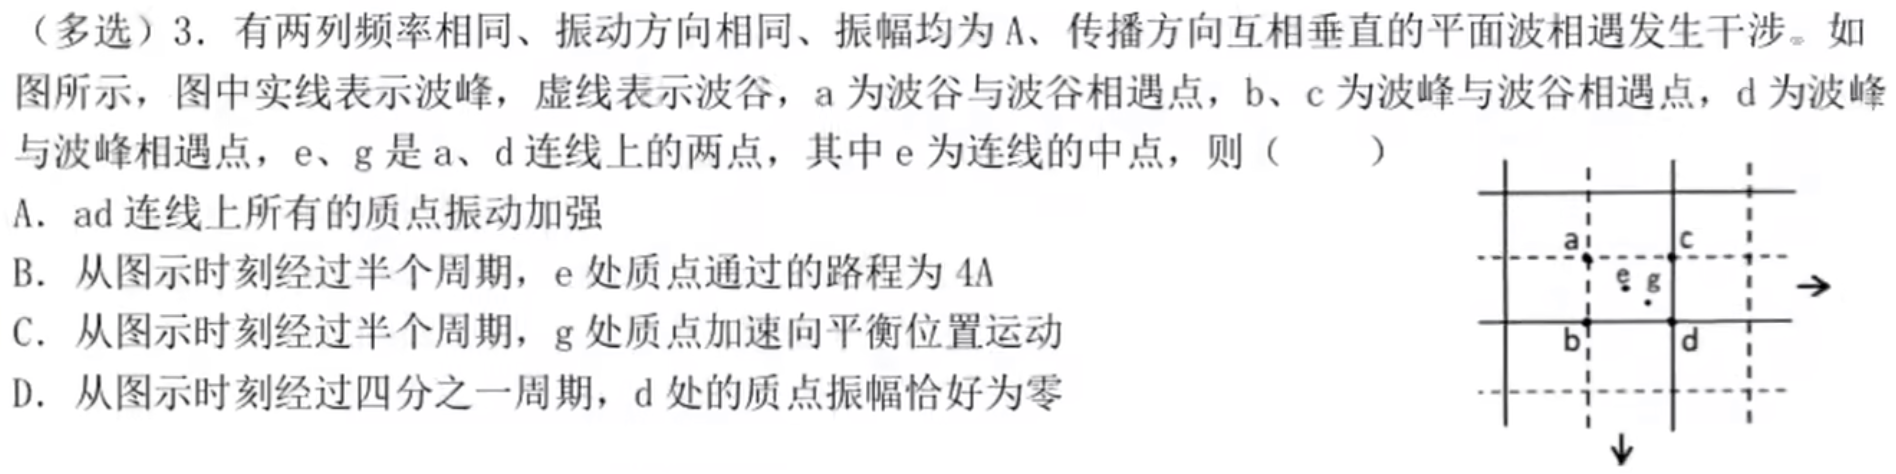
\includegraphics[width = 0.95\textwidth]{./pictures/2.1-3.png}

\begin{itemize}
    \item 正解:\quad ABC
    \item 总结:\quad
          \begin{itemize}
              \item[A.] 两个振幅加强点的连线上的所有点都是加强点.
              \item[B.] 简谐运动的结论,经过一个周期,质点(平衡位置或最大振幅位置)走过路程为4倍振幅.
                  经过半个周期,质点走过2倍振幅.在此选项中,质点$e$为加强点振幅为$2A$,经过半个周期,质点走过$2*2A = 4A$
              \item[C.] 运用简谐波的结论和同侧法判断振动方向(当然题目存在一定的语言上的细节,$g$减速到最大振幅后向平衡位置移动,加速度指向平衡位置)
              \item[D.] 题目考查的语言的艺术,可以描述$d$点所处位置为平衡位置,但是$d$点是振幅加强点不为$0$
          \end{itemize}
\end{itemize}

\vspace{2em}

\subsubsection{II-2:斜面弹簧组合体简谐振子}
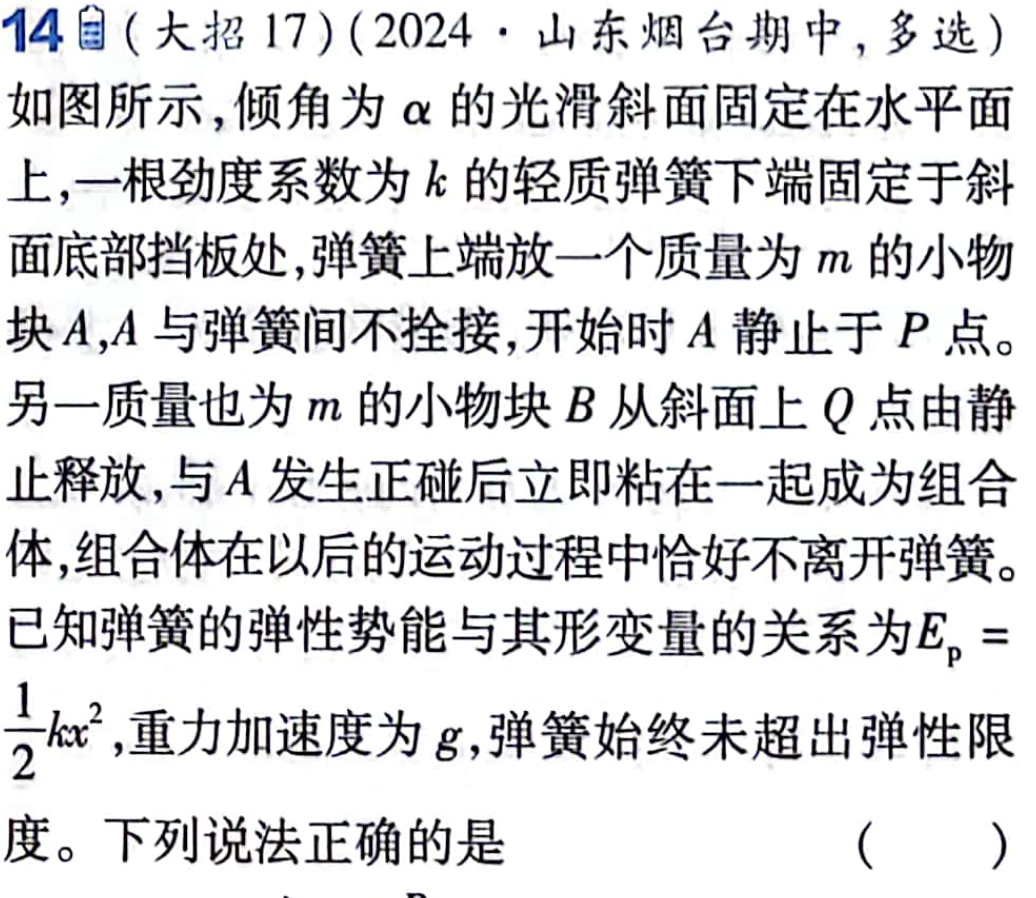
\includegraphics[width = 20em]{./pictures/2.1-7.png}
\hspace{2em}
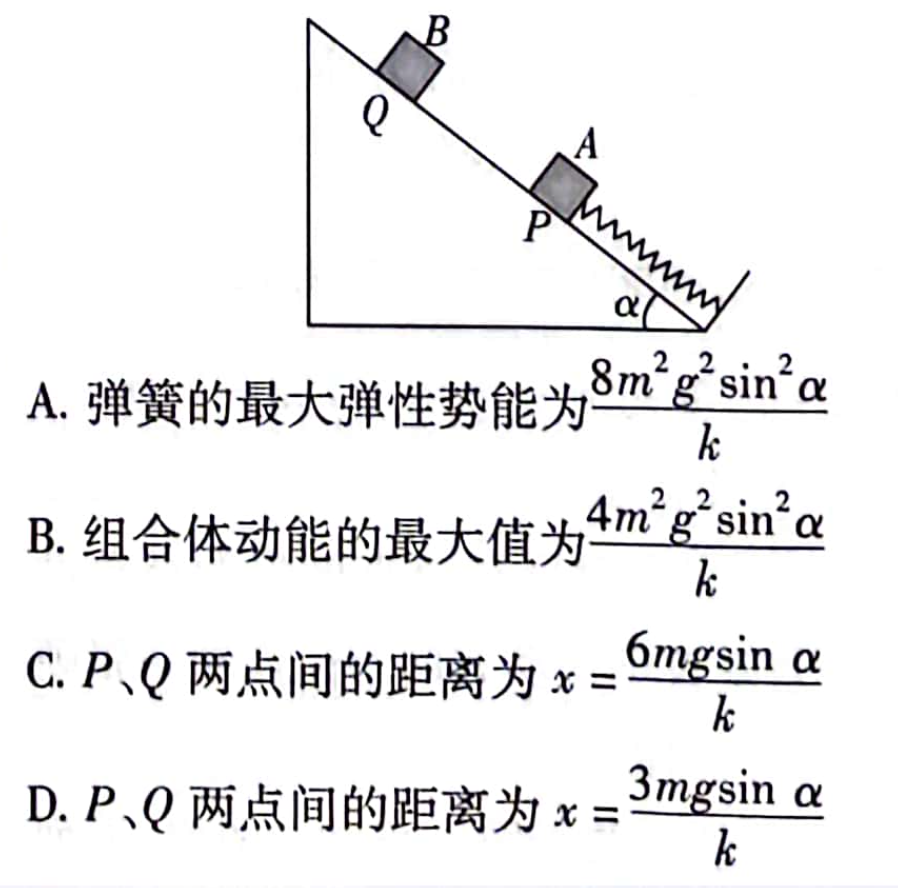
\includegraphics[width = 20em]{./pictures/2.1-8.png}

\begin{itemize}
    \item 正解:AD
    \item 总结:
          题目的过程较为复杂,我们需要理清每一个阶段
          \begin{enumerate}
              \item 初始阶段,物块$A$静止,弹簧被压缩至$x_{1} = \frac{mg\sin{\alpha}}{k}$
              \item 组合体阶段,题目的关键信息:组合体运动过程中\textbf{恰好}不离开弹簧,因此在恢复原长时组合体的速度为$0$.此时的回复力$F_{\text{回}} = 2mg\sin{\alpha}$(向下),
                    由简谐振动的性质,压缩到最大时的回复力大小也应该如此,因此$kx_{2} - 2mg\sin{\alpha} = 2mg\sin{\alpha} \quad \lra \quad x_{3} = \frac{4mg\sin{\alpha}}{k}$.

                    由此可得弹簧的最大弹性势能$ E_{pmax} = \frac{1}{2}kx_{2}^{2} = \frac{8m^{2}g^{2}\sin^{2}{\alpha}}{k} = 8J \quad (J = \frac{m^{2}g^{2}\sin^{2}{\alpha}}{k} )$

              \item 研究组合体最大的动能,显然我们需要找到谐振运动的平衡点即$F_{\text{回}} = 0$的位置$x_{2} = \frac{2mg\sin{\alpha}}{k} $.

                    因此在组合体从弹簧原长位置到平衡位置的过程中,弹簧弹性势能增加量$ \triangle E_{p} = 2J $,重力势能的减少量$ \triangle E_{g}2mgx_{2}\sin{\alpha} = 4J $ ,所以组合体的动能为$2J$

              \item 计算$PQ$距离重要在于研究初始位置$x_{1}$的碰撞问题得到速度,碰撞后成为组合体的动量守恒问题比较简单$ mv = 2mv^{'} \quad v^{'} = \frac{v}{2} $.组合体的速度从初始位置压缩到最大位置$x_{3}$(速度变为$0$),
                    其中重力势能的减少量$ \triangle E_{g} = 2mg(x_{3} - x_{1})\sin{\alpha} = 6J$,弹簧弹性势能的增加量$ \triangle E_{p} = 8J - \frac{1}{2}J  = \frac{15}{2}J$,所以组合体的初动能为$\frac{3}{2}J$,因策
                    得到$v^{'} = \sqrt{\frac{3mg^{2}\sin^{2}{\alpha}}{2k}} \quad \lra \quad v = 2 v^{'} \quad mgx_{PQ}\sin{\alpha} = \frac{1}{2}mv^{2} \quad x_{PQ} = \frac{3mg\sin{\alpha}}{k} $
          \end{enumerate}
\end{itemize}


\vspace{2em}

\subsubsection{IV-1:干涉计算}
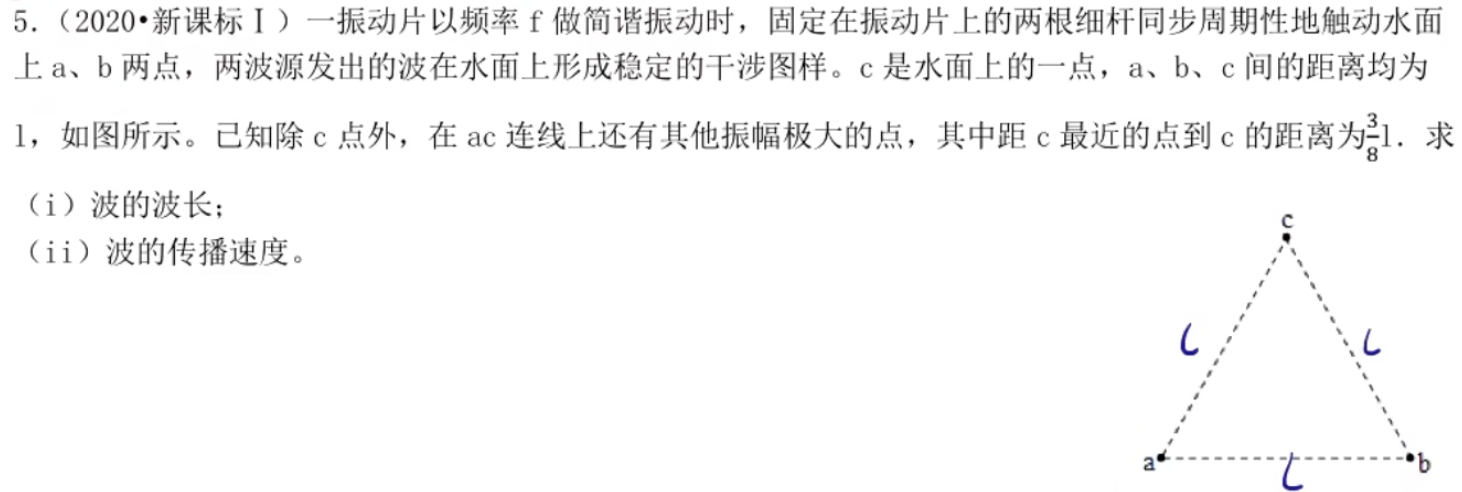
\includegraphics[width = 0.95\textwidth]{./pictures/2.1-4.png}

\begin{itemize}
    \item 正解:\quad $(1)\,\frac{1}{4}L \quad (2)\,\frac{1}{4}fL$
    \item 总结:\quad 需要理清波源为哪两个点,同时找到某个振动加强点(多少个$\lambda$)到波源的两个距离,余弦定理做计算.
    \item 扩展:\quad 三角函数相关
          \begin{formal}
              \begin{itemize}
                  \item 展开
                        $$ \sin{(\theta \pm \beta)} = \sin{\theta}\cos{\theta} \pm \cos{\theta}\sin{\theta} $$
                        $$ \cos{(\theta \pm \beta)} = \cos{\theta}\cos{\theta} \mp \sin{\theta}\sin{\theta} $$
                        $$ \tan{(\theta \pm \beta)} = \dfrac{\tan{\theta} \pm \tan{\beta}}{1 \mp \tan{\theta}\tan{\beta}}$$

                  \item 余补关系
                        $$ \sin{(\pi - \theta)} = \sin{\theta} \quad \cos{(\pi - \theta)} = - \cos{\theta} \quad \tan{(\pi - \theta)} = -\tan{\theta}$$

                        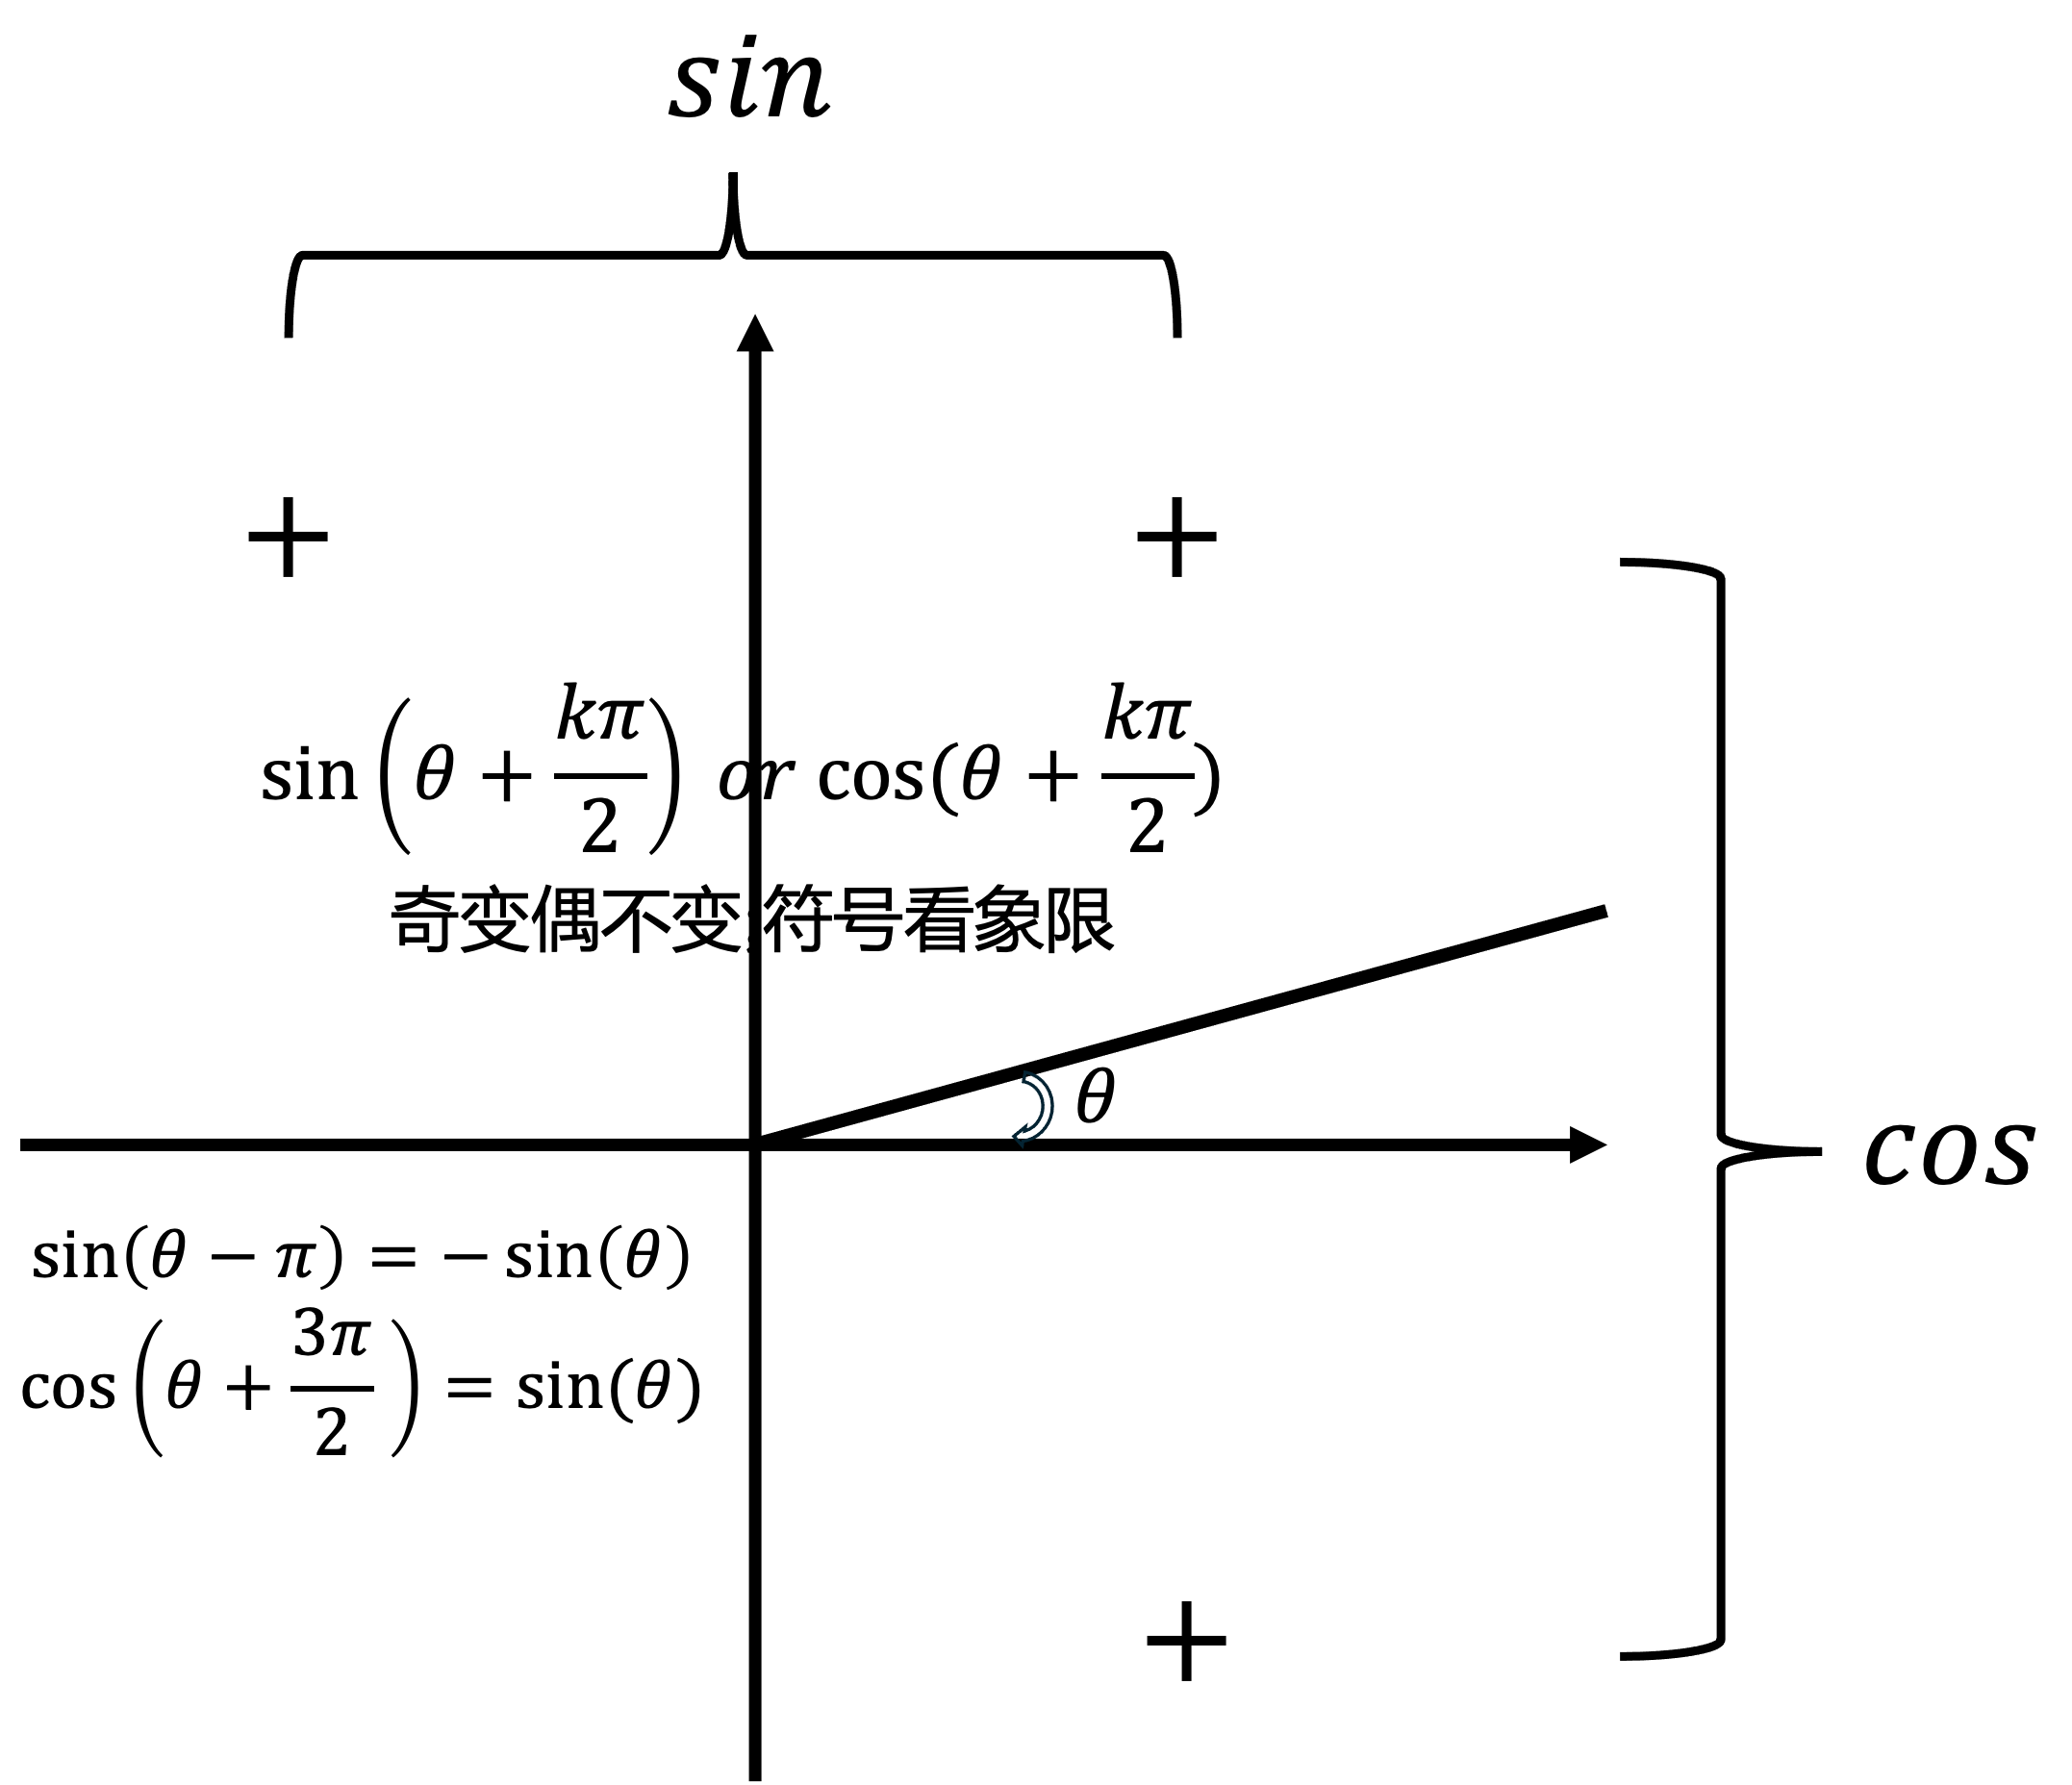
\includegraphics[width = 20em]{./pictures/2.1-5.png}

                  \item 正弦定理
                        $$ \dfrac{a}{\sin{\alpha}} = \dfrac{b}{\sin{\beta}} = \dfrac{c}{\sin{\gamma}}   $$

                  \item 余弦定理
                        $$ \cos{\gamma} = \dfrac{a^{2}+b^{2} - c^{2}}{2ab} $$

                  \item 二倍角
                        $$ \sin{2\theta} = 2\sin{\theta}\cos{\theta} \quad \cos{2\theta} = \cos^{2}{\theta} - \sin^{2}{\theta} \quad \tan{2\theta} = \dfrac{2\tan{\theta}}{1-\tan^{2}{\theta}}$$

                  \item 降次
                        $$ \sin^{2}{\theta} = \dfrac{1 - \cos{2\theta}}{2} \quad \cos^{2}{\theta} = \dfrac{1 + \cos{2\theta}}{2} \quad \tan^{2}{\theta} = \dfrac{1-\cos{2\theta}}{1+\cos{2\theta}}$$
              \end{itemize}
          \end{formal}
\end{itemize}

\vspace{2em}

\subsection{原子核物理}
\subsubsection{I-1: 不同原子核的平均值质量和}
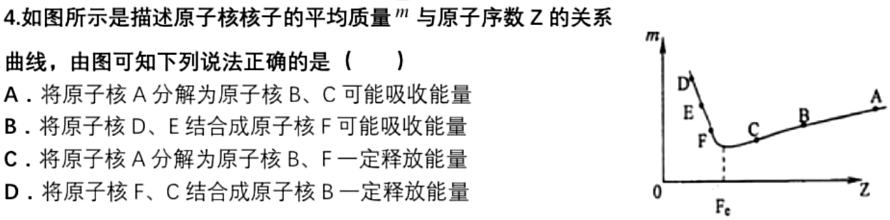
\includegraphics[width = 0.95\textwidth,keepaspectratio]{./pictures/2.2-1.png}

\begin{itemize}
    \item 正解:\quad C
    \item 总结:\quad 质量亏损释放能量,质量增大吸收能量

          \hspace{3.3em}在计算某两种元素原子核的平均质量时,并不是简单的加和

          \hspace{3.3em}例如$B \, C$两种元素混合后其平均质量值应该介于两者之间.
\end{itemize}

\vspace{2em}

\subsubsection{II-1: 比结合能大小与能量吸收释放}
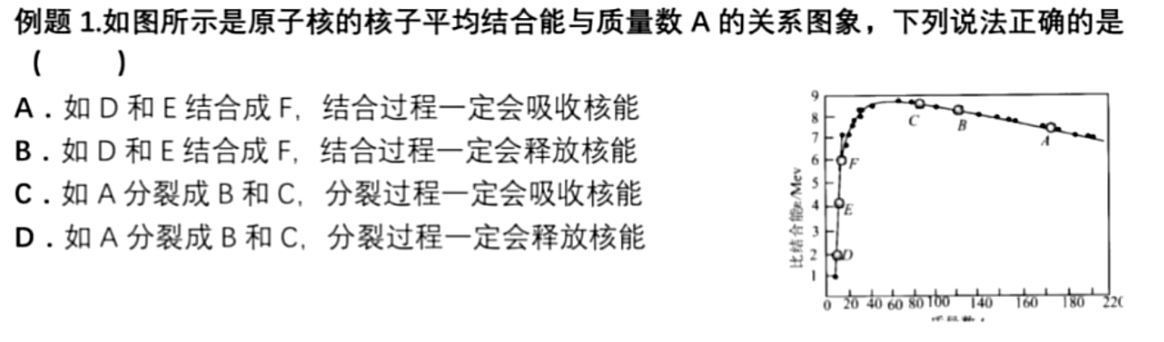
\includegraphics[width = 0.95\textwidth,keepaspectratio]{./pictures/2.2-2.png}

\begin{itemize}
    \item 正解:\quad BD
    \item 总结:\quad 比结合能越大则原子核状态更稳定,具备更低的能量状态.因此当比结合能上升时释放能量

          \hspace{3.3em}多元素的比结合能的计算类同理与平均质量
\end{itemize}

\subsection{热力学}
\subsubsection{I-1: 三管连通器}
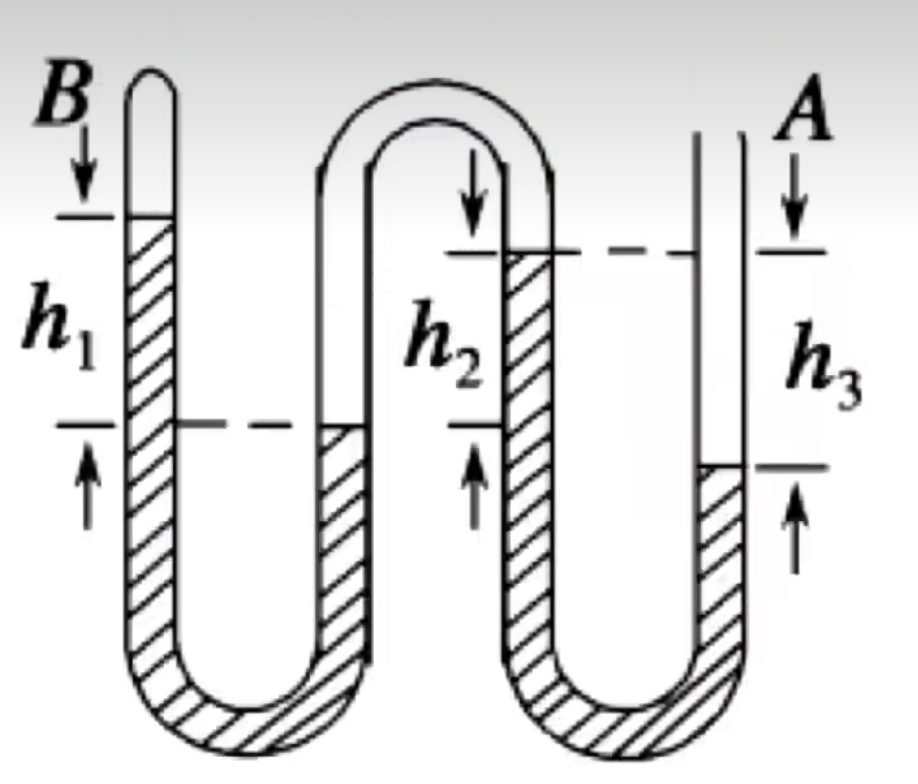
\includegraphics[width = 0.3\textwidth,keepaspectratio]{./pictures/2.3-1.png}
\begin{itemize}
    \item 正解:\quad $P_{B} = P_{A} + \rho g (h_{3} - h_{1}) $
    \item 总结:\quad 前两管: $ P_{B} + \rho g h_{1} = P_{C}\text{,后两管} P_{C} + \rho g h_{3} = P_{0}$

\end{itemize}

\vspace{2em}

\subsubsection{I-2: 液泡上浮问题}
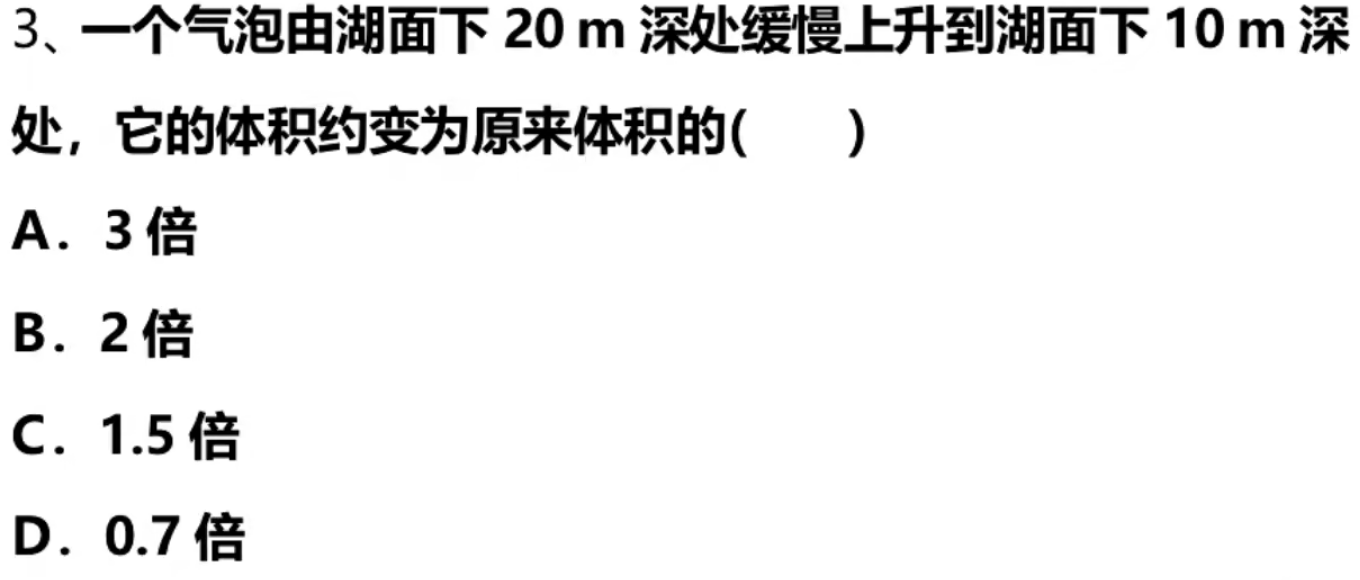
\includegraphics[width = 0.55\textwidth,keepaspectratio]{./pictures/2.3-2.png}

\begin{itemize}
    \item 正解:\quad C
    \item 总结:\quad 外界大气压的作用应该被计算进去
\end{itemize}

\vspace{2em}

\subsubsection{I-3: 图像计算}
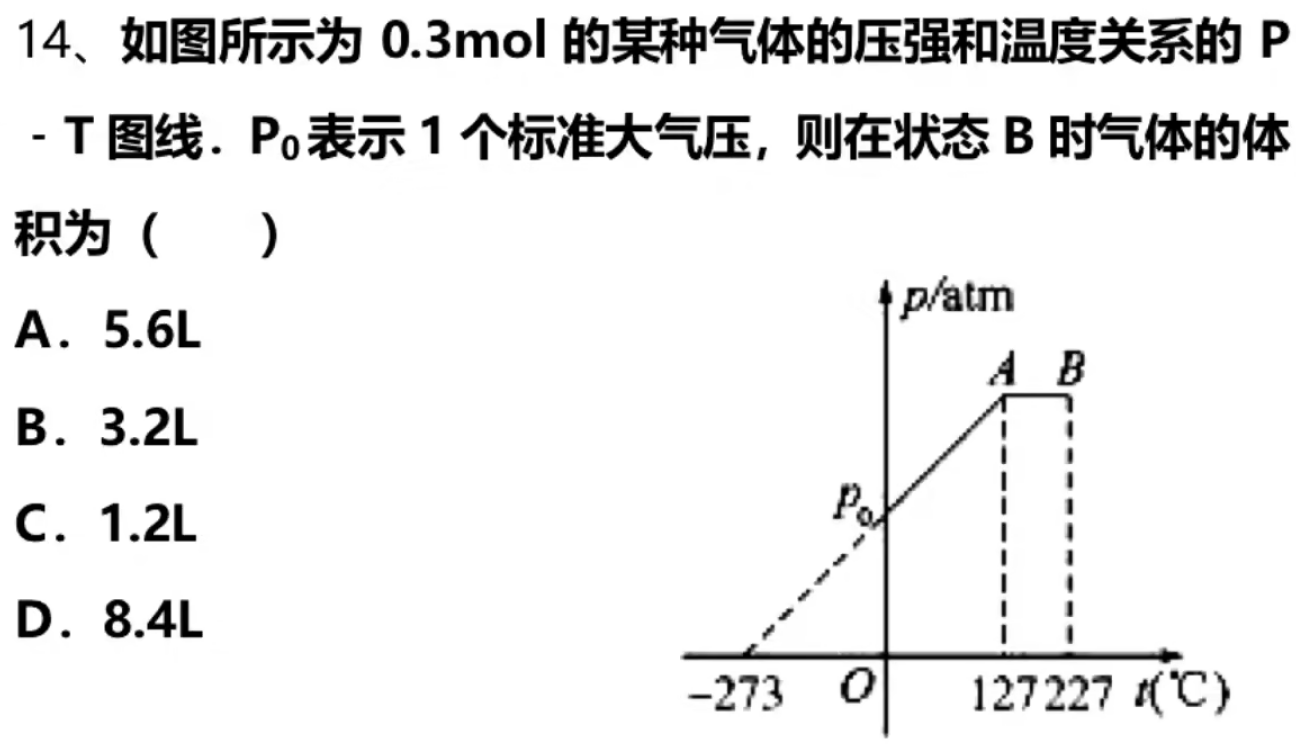
\includegraphics[width = 0.55\textwidth,keepaspectratio]{./pictures/2.3-3.png}

\begin{itemize}
    \item 正解:\quad D
    \item 总结:\quad 首先应该向左平移$y$轴,使得横坐标换算成开尔文温度.

          \hspace{3.3em}新的坐标系下,斜线$OA$满足$P = \frac{C}{V}T$斜率为定值,因此为等容过程.

          \hspace{3.3em}$T = 273k$时过$P_{0}$,此时气体体积为$22.4L$,因此$V_{A} = 22.4L$,横线$A \ra B$为等压过程,计算温度只比即可求得$V_{B}$
\end{itemize}

\vspace{2em}

\subsubsection{I-4: 液柱动力学问题}
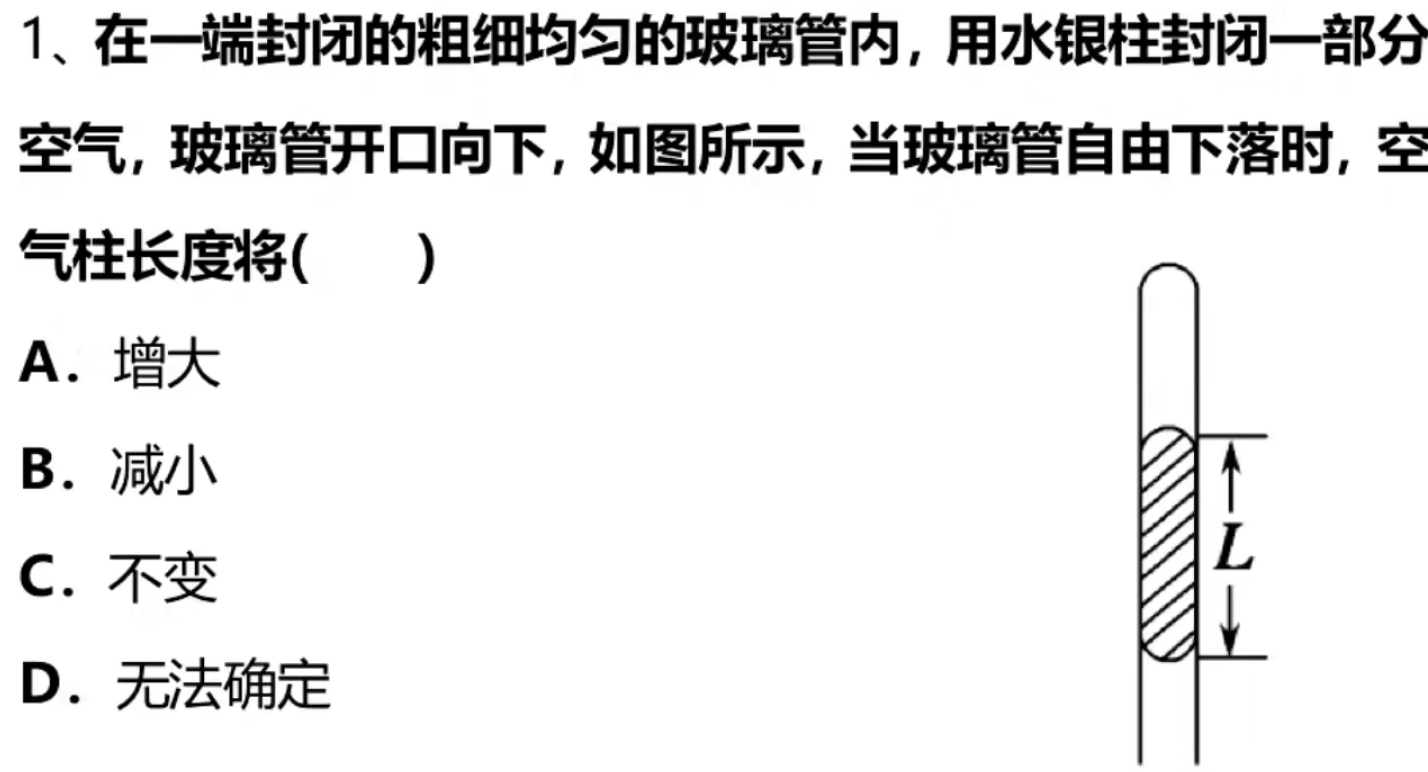
\includegraphics[width = 0.55\textwidth,keepaspectratio]{./pictures/2.3-4.png}

\begin{itemize}
    \item 正解:\quad B
    \item 总结:\quad 动力学问题主要在于分析好初末态,同时列受力分析方程.

          \hspace{3.3em}初态$PS + mg = P_{0}S$,末态自由落体加速度为$g$

          \hspace{3.3em}$P^{'}S + mg - P_{0}S = ma = mg \lra P^{'} = P_{0}$液柱上方压强增大,因此液柱上方体积减小
\end{itemize}

\vspace{2em}

\subsubsection{I-5: 两气挤压问题}
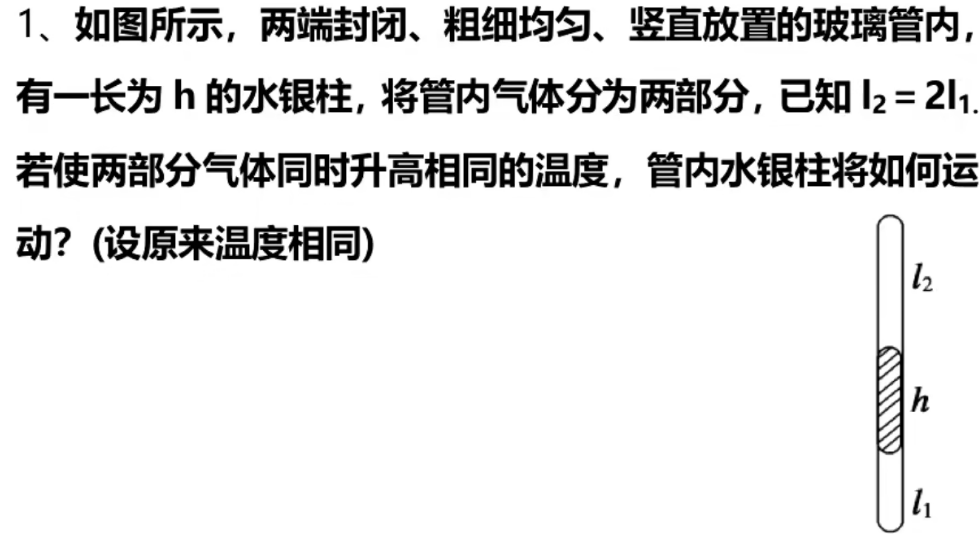
\includegraphics[width = 0.55\textwidth,keepaspectratio]{./pictures/2.3-5.png}

\begin{itemize}
    \item 正解:\quad 向上移动
    \item 总结:\quad 三个状态参量中,真正使得液柱移动的物理量是$P$,在查理定律中$\frac{P}{T} = \frac{C}{V}$

          \hspace{3.3em}升温瞬间可视为等体过程,因此函数为过原点的直线可得$\frac{P}{T} = \frac{\triangle P}{\triangle T}$

          \hspace{3.3em}$ \triangle P_{1} = \frac{P_{1}}{T_{1}} \triangle T = \frac{C}{V_{1}} \triangle T $

          \hspace{3.3em}$ V_{2} = 2 V_{1}  \quad \lra \triangle P_{1} > \triangle P_{2}$
\end{itemize}





\vspace{2em}

\section{高三}

\subsection{2023届巴蜀中学高考适应性月考(十)}
\subsubsection{I-6:同步卫星}
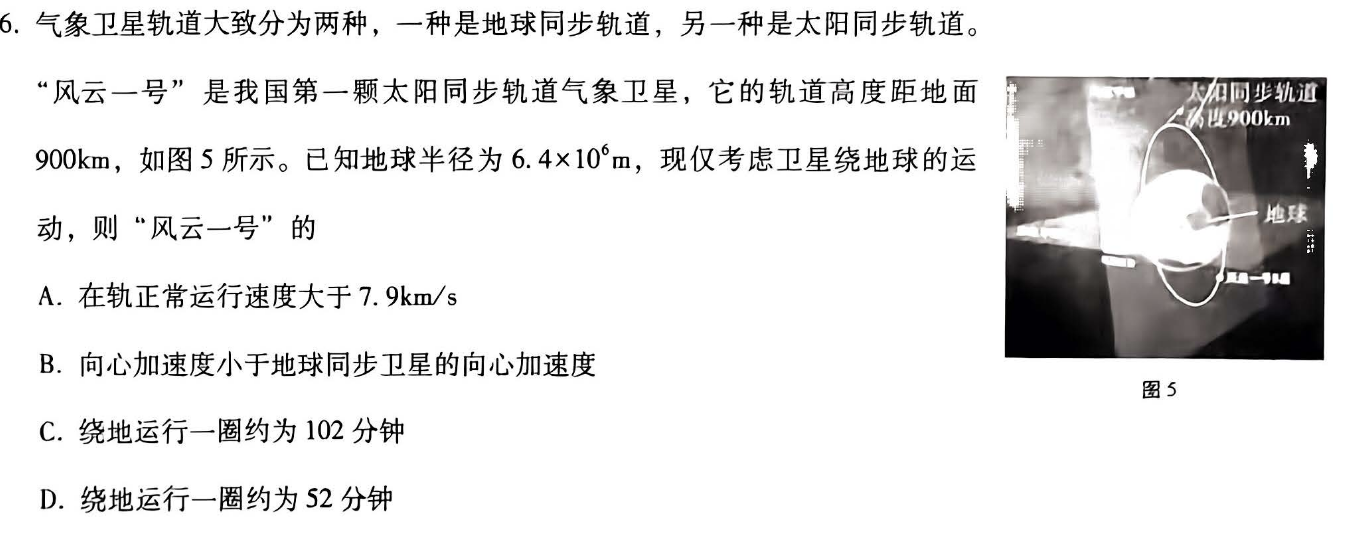
\includegraphics[width = 0.95\textwidth,keepaspectratio]{./pictures/3.1-1.png}

\begin{itemize}
    \item 正解:\quad C
    \item 总结:\quad
          \begin{itemize}
              \item 近地卫星:其\textbf{运动轨道半径约为地球半径},因此为\textbf{最大的环绕速度$7.9km/s$},周期为85分钟(不用记忆)
              \item 同步卫星:其\textbf{周期与地球自转相同为$24h$}
          \end{itemize}
    \item 扩展:第三与四个选项的计算需要知道两个竖数值中的一个
          \begin{itemize}
              \item 同步卫星的轨道高度为$3.6 \cross 10^{7} m$,然后用开普勒第三定律
                    \begin{thm*}
                        开普勒行星运动定律(不用纠结证明)
                        \begin{itemize}
                            \item 第一定律:行星运动在椭圆轨道上,太阳处于椭圆的焦点上
                            \item 第二定律:行星与太阳的连线在相同时间内扫过的面积相等
                            \item 第三定律:$\frac{a^{3}}{T^{2}} = k$
                        \end{itemize}
                    \end{thm*}
              \item 近地卫星的周期为$85$分钟,根据第三定律得知太阳同步轨道卫星的周期至少大$85$分钟,因此选$C$
          \end{itemize}
\end{itemize}

\vspace{2em}

\subsubsection{II-1:简谐波的图像问题}
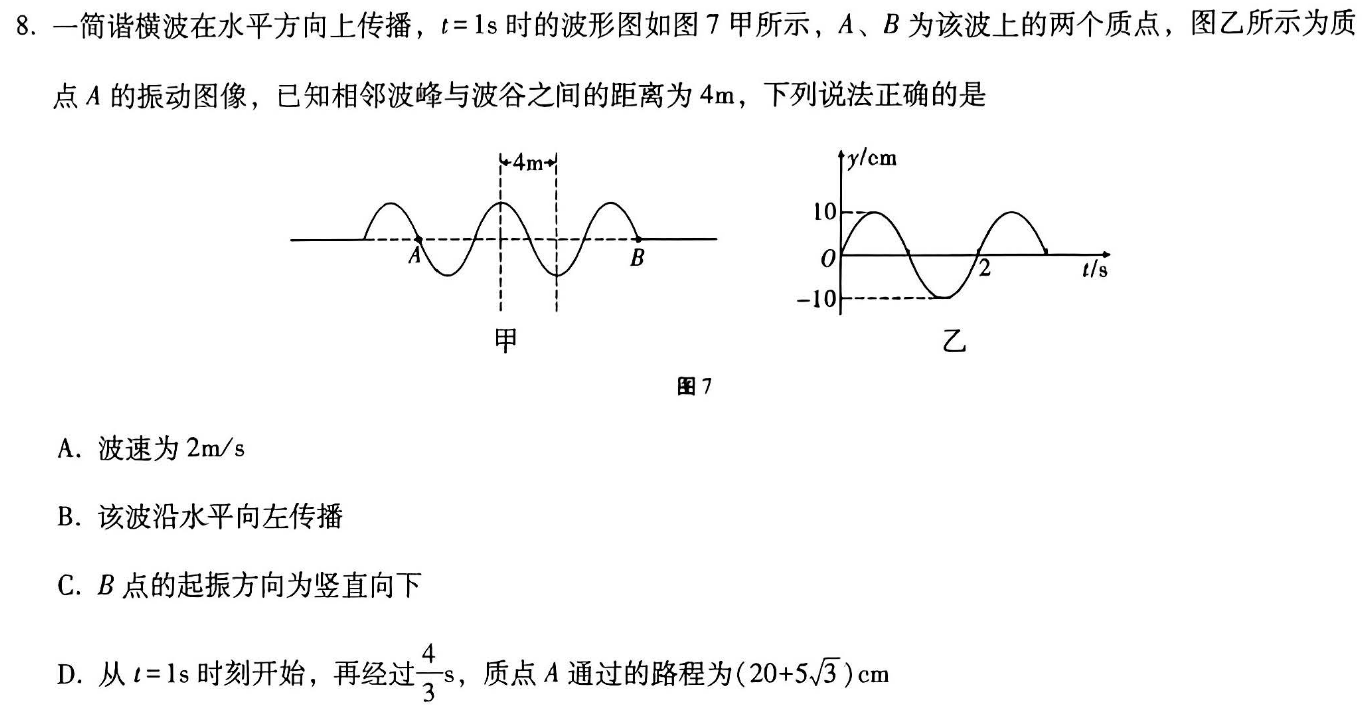
\includegraphics[width=0.95\textwidth,keepaspectratio]{./pictures/3.1-2.png}

\begin{itemize}
    \item 正解:\quad BD
    \item 总结:\quad 选项$C$问的是起振($t=0s$)方向,而题目\textbf{图乙}是给的$t=1s$的质点振动图\\
          选项$D$需要求$t=\frac{1}{3}s$时对应的$y$值,所以需要根据图像中已知数据点求解三角函数的具体表达式
\end{itemize}

\begin{proof}
    设$ y = 10 \sin{\omega t + \phi_{0}}$
    \begin{align*}
        t & = 0s \quad \sin{\phi_{0}} = 0 \lra \phi_{0} = 0                           \\
        t & = 1s \quad \sin{\omega} = 0 \lra \omega = n\pi                            \\
        t & = \frac{1}{2}s \quad \sin{\frac{\omega}{2}} = 1 \lra \omega = \pi + 4n\pi
    \end{align*}
\end{proof}
$$
    y = 10\sin{\pi t} \quad t = \frac{1}{3}s \lra y = 10 \vdot \frac{\sqrt{3}}{2} = 5\sqrt{3}
$$

\vspace{2em}

\subsubsection{II-3:动生电动势的平均值问题}
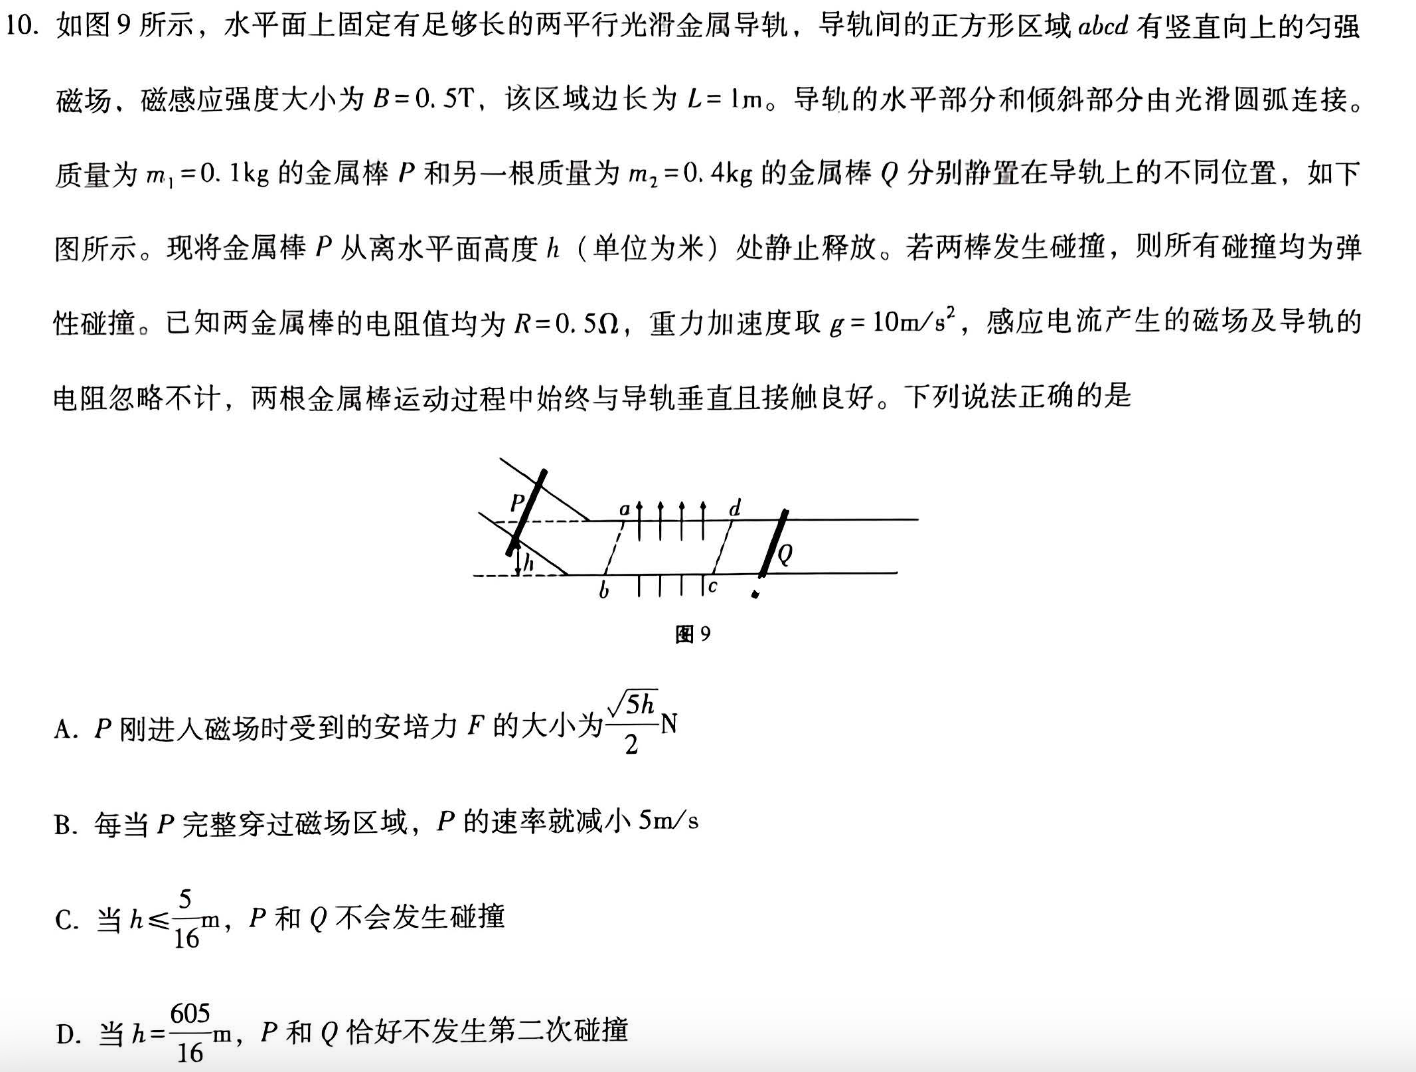
\includegraphics[width=0.95\textwidth,keepaspectratio]{./pictures/3.1-3.png}

\begin{itemize}
    \item 正解:\quad ACD
    \item 总结:\quad 选项B, $E = - \frac{\triangle \Phi}{\triangle t}$,在高中阶段$\triangle t$比较小的时候为瞬时
          电动势,当$\triangle t$比较大的时候,即为一个过程量得到的是$\overline{E}$,因此可以得到$\overline{I},\overline{F}$
          \begin{align*}
              \varepsilon         & = \frac{\triangle \Phi}{\triangle t} = \frac{B \vdot \triangle S}{\triangle t} \\
              I                   & = \frac{\varepsilon}{2R} = \frac{B}{2R} \vdot \frac{\triangle S}{\triangle t}  \\
              F                   & = B I L = \frac{B^{2}L \triangle S}{2R \vdot \triangle t}                      \\
              F \vdot \triangle t & = \frac{B^{2} L \triangle S}{2 R} = m(v_{t} - v_{0})
          \end{align*}
          复杂变化的安培力对导体棒的冲量,仅仅与面积的改变量有关$\lra$速度的变化量仅与走过的面积有关 \\
          选项D,恰好不能第二次碰撞即再次扫过2次磁场面积后速度为球2第一次碰后速度
\end{itemize}

\vspace{2em}

\subsubsection{IV-1:均匀滴落的沙漏问题}
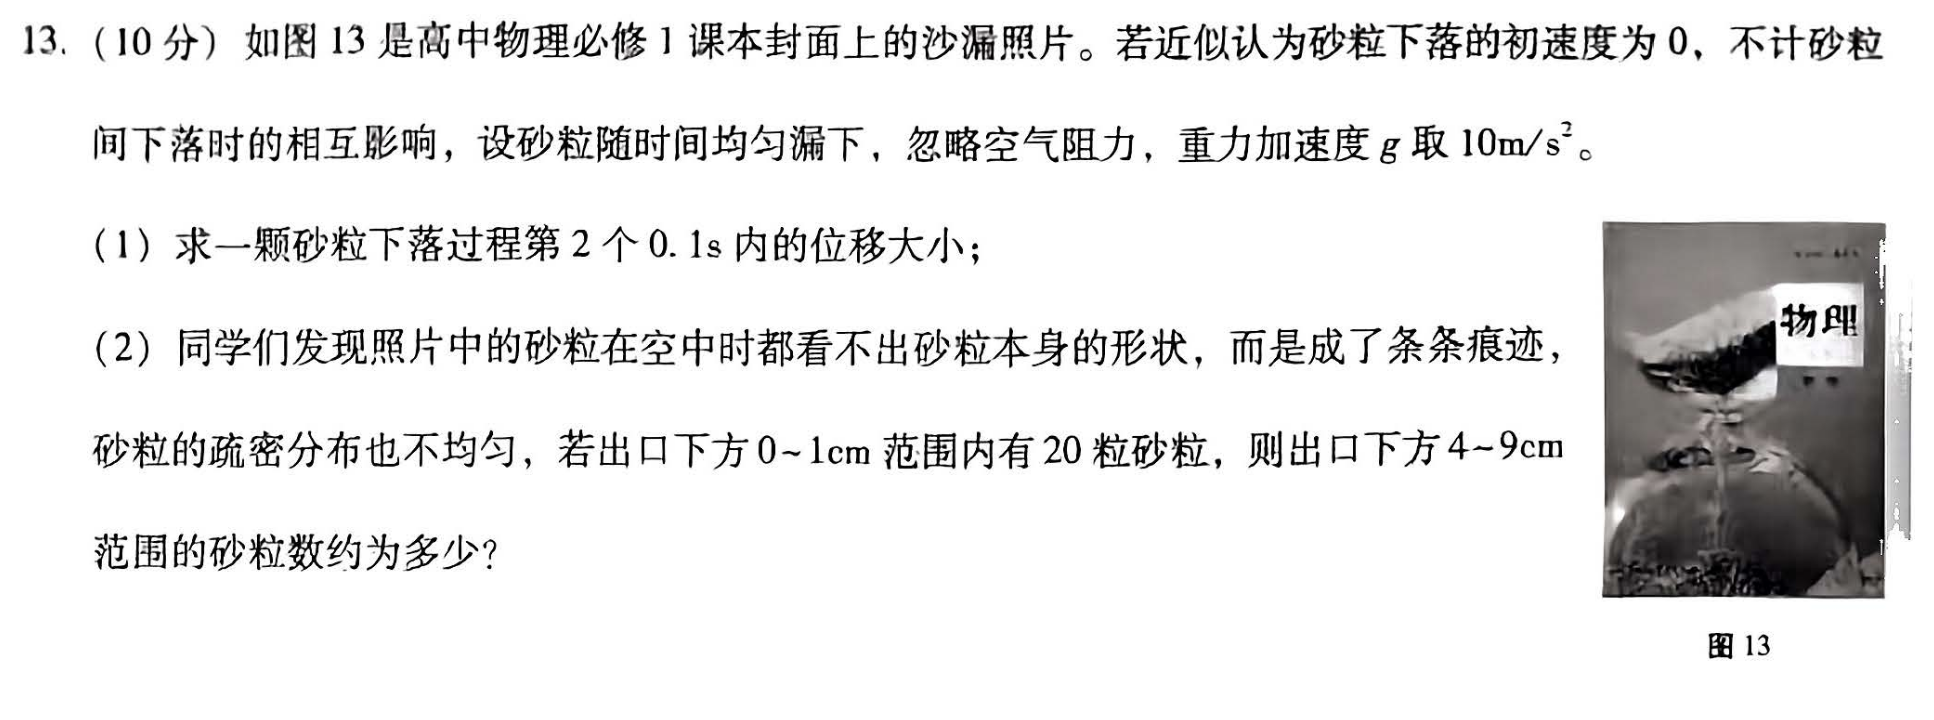
\includegraphics[width=0.95\textwidth,keepaspectratio]{./pictures/3.1-4.png}

\begin{itemize}
    \item 总结:好题收藏,第二问关键在与「沙粒随时间均匀漏下」,从已知条件中求出\textbf{沙粒平均流量},计算第二段的时间长度即可
\end{itemize}

\vspace{2em}


\subsubsection{IV-2:折射率几何大题}
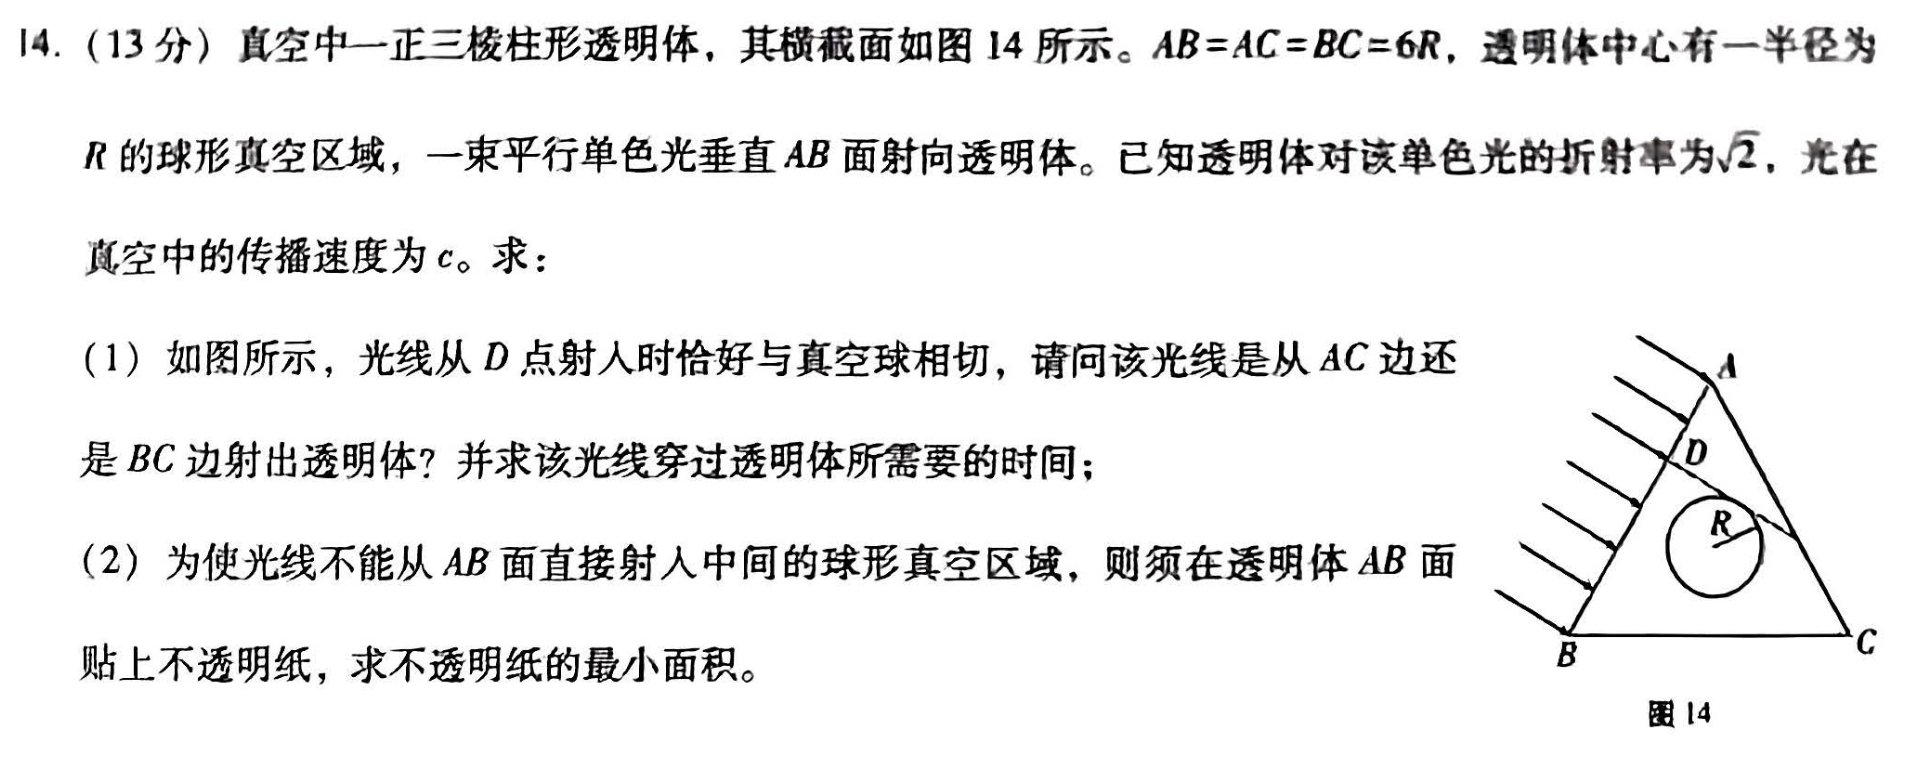
\includegraphics[width=0.95\textwidth,keepaspectratio]{./pictures/3.1-5.png}

\begin{itemize}
    \item 总结:第一问当光垂直入射介面交界处 or 平行入射介面交界处,光路沿原方向继续传播
    \item 第二问不难,即光线接触真空区域时,以临界角$\frac{\pi}{2}$射入,值的思考的是遮挡面积是一个圆形域
\end{itemize}

\vspace{2em}

\subsubsection{IV-3:磁聚焦+区域面积问题}
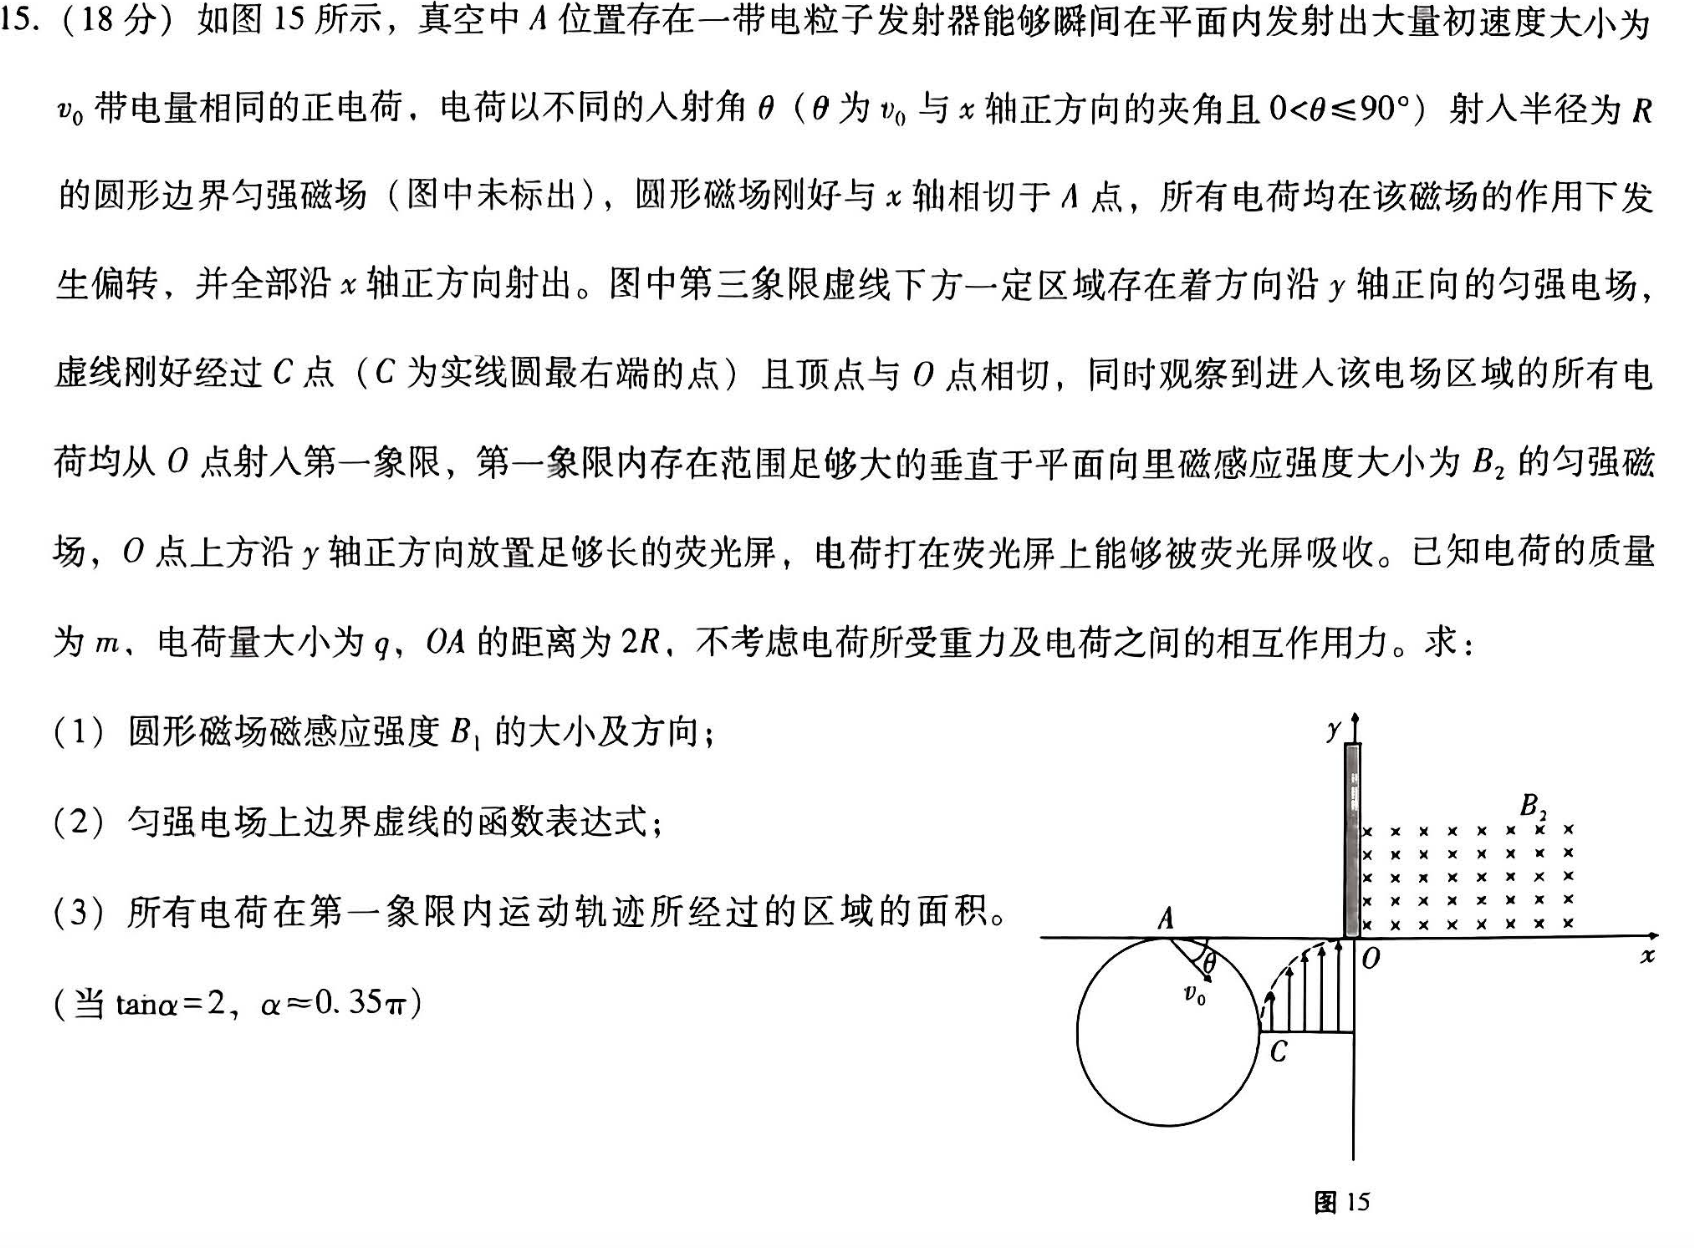
\includegraphics[width=0.95\textwidth,keepaspectratio]{./pictures/3.1-6.png}

\begin{itemize}
    \item 总结:\quad 第一问考的\textbf{磁聚焦}(证明通过相似三角形),粒子旋转半径刚好为磁场半径$R$,也可以取特殊角度$\frac{\pi}{2}$
          \begin{figure}[h]
              \centering
              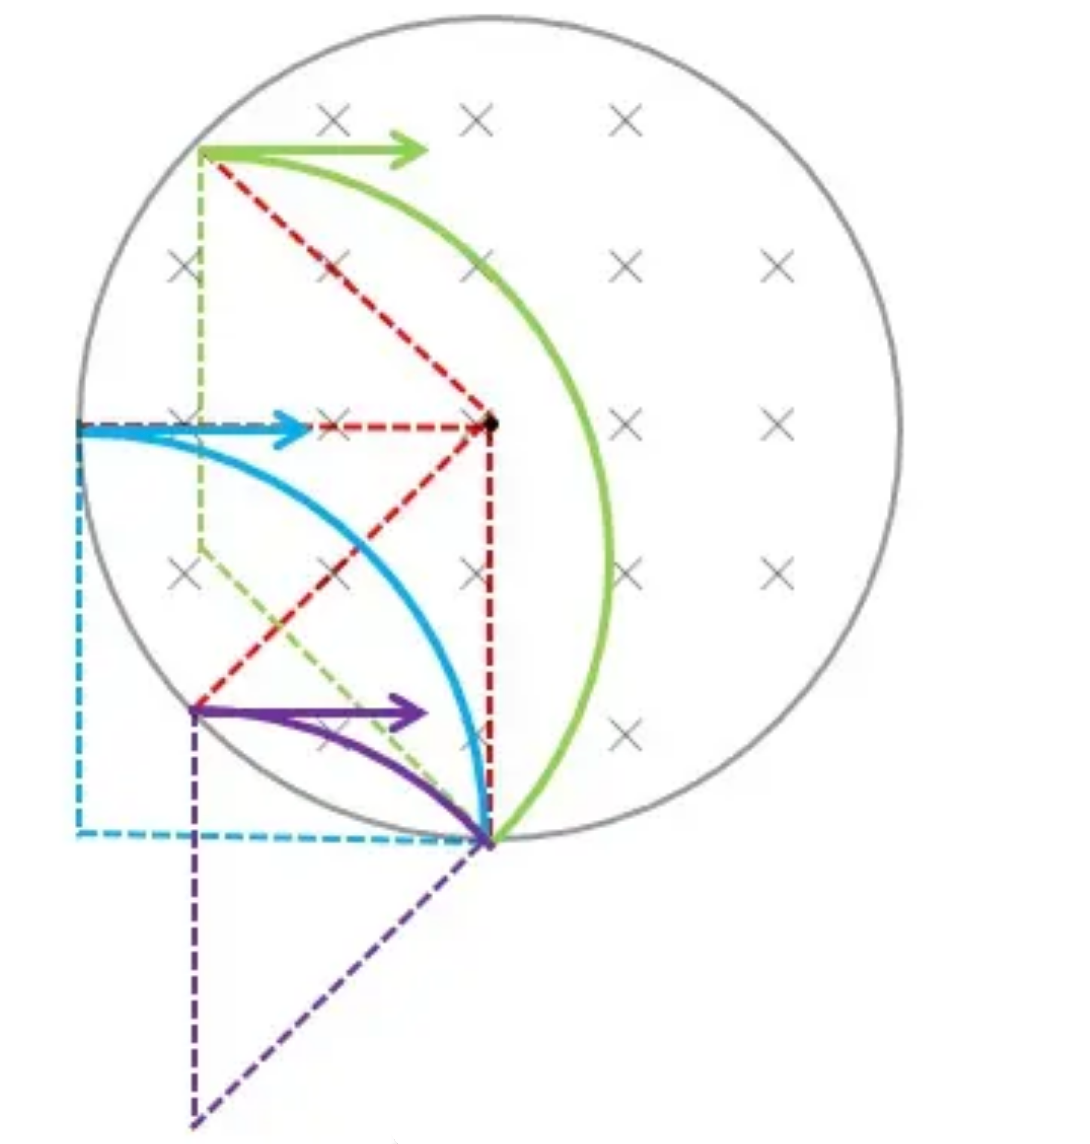
\includegraphics[width=20em,keepaspectratio]{./pictures/3.1-7.png}
          \end{figure}
    \item 第二问不难,注意电场需要求出来,设射入电场的粒子$(x_{0},y_{0})$,位移为坐标的负数.$E = \frac{2mv^{2}}{qR} \quad y = - \frac{1}{R} x^{2}$
    \item 第三问比较特殊,需要设$h$(距离下$x$轴的距离),去求不同高度下打到$y$轴上点的坐标,设进入第二磁场区域的速度方向与$x$轴成$\theta$角,打击点$ y = 2 r \cos{\theta}$
          $$
              \cos{\theta} = \frac{1}{\sqrt{1 + \frac{4h}{R}}} = 1 \quad \quad \quad r = \frac{mv}{qB_{2}} = \frac{mv_{0} \sqrt{1+\frac{4h}{R}}}{q B_{2}} = \frac{mv_{0} k}{qB_{2}}
          $$
          $$
              2 r \cos{\theta} = \frac{2mv_{0}}{qB_{2}}
          $$
          因此不同速度的粒子打在$y$轴上的点为同一点
          $$
              h = 0 \lra r_{0} = \frac{mv_{0}}{qB_{2}} \quad \quad \quad h = R \lra r_{1} = \frac{\sqrt{5} m v_{0}}{qB_{2}} \quad \theta = 0.35\pi
          $$
          \begin{align*}
              S_{0} & = \frac{1}{2} \vdot \pi r_{0}^{2} = \frac{\pi}{2} \vdot (\frac{mv_{0}}{qB_{2}})^{2}                                                           \\
              S{1}  & = \pi r_{1}^{2} (\frac{\pi - 2\theta}{2 \pi}) - r_{1}^{2} \sin{\theta} \cos{\theta} = (\frac{3\pi}{4} - 2) \vdot (\frac{m v_{0}}{qB_{2}})^{2} \\
              S     & = S_{0} - S_{1} = (\frac{8-\pi}{4}) \vdot (\frac{m v_{0}}{qB_{2}})^{2}
          \end{align*}
\end{itemize}

\vspace{2em}

\subsection{2024八中高考适应性月考(六)}
\subsubsection{I-1:万有引力航天}

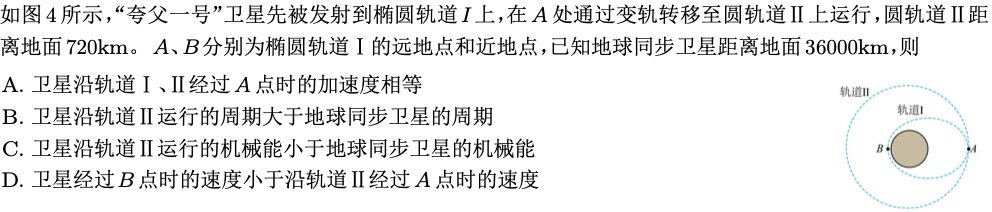
\includegraphics[width=0.95\textwidth,keepaspectratio]{./pictures/3.2-1.png}

\begin{itemize}
    \item 正解: A
    \item 总结: 正确选项容易选出,仅需要判断此时的万有引力的大小,没有涉及变轨时的加减速.选项$C$的引力势能的计算是$E_{p} = - \frac{GmM}{R}$.
          但是这里注意是两个卫星的机械能比较,无法知道质量关系(易错点)
\end{itemize}

\vspace{2em}

\subsubsection{I-2:势能计算}
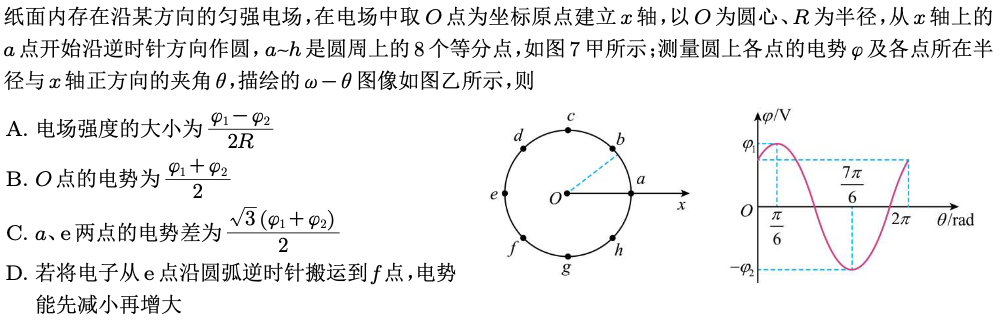
\includegraphics[width=0.95\textwidth,keepaspectratio]{./pictures/3.2-2.png}

\begin{itemize}
    \item 正解: C
    \item 总结: 比较有新意的一道题,重点在于找到等势能的两点并连接,$\varphi_{1} \, \varphi_{2}$的大小位置,应该根据对称性计算出$\varphi = 0$
          的两个位置的角度为$\frac{2\pi}{3} \, \frac{5\pi}{6} $,由此可以得到电场线的方向.
\end{itemize}

\vspace{2em}

\subsubsection{II-1:纯电阻动生电动势杆模型}
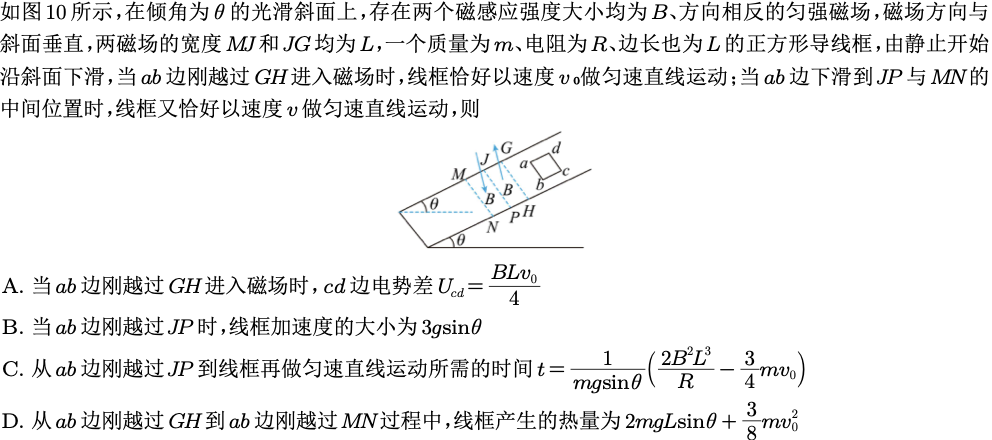
\includegraphics[width=0.95\textwidth,keepaspectratio]{./pictures/3.2-3.png}

\begin{itemize}
    \item 正解: BC
    \item 总结: 注意有两个磁场区域均在切割.$C$选项需要求得第二个匀速运动的速度大小$\frac{1}{4}v_{0}$在根据动量定理(平均值法)计算时间.
          选项$D$使用动能定理即可
\end{itemize}

\vspace{2em}

\subsubsection{IV-1:变质量多次碰撞与数列}
\includegraphics[width=0.95\textwidth,keepaspectratio]{./pictures/3.2-4.png}

\begin{itemize}
    \item 正解: \begin{enumerate}[label = (\arabic*)]
              \item $60N$
              \item $\sqrt{2} \, m \slash s$
              \item $E_{kn0} = \frac{1}{n} E_{k10} - \frac{2^{2} + 3^{2} + \cdots n^{2}}{n} mg\mu d$
          \end{enumerate}
    \item 总结: 重点在于第三问,每次质量碰撞后会发生改变,这会影响每一阶段的动量定理以及摩擦力做功

          \hspace{3em}得到递推公式后变成数学问题

          \begin{align*}
                                & \text{假设第}n-1\text{次碰撞后的动能为}  E_{k(n-1)1}\text{,此时有}n\text{个物块粘黏}                      \\
              E_{kn0}           & = E_{k(n-1)1} - nmg\mu d                                                               \\
                                & \text{研究第}n-1\text{次碰撞过程}     \text{,物块由}n-1\text{个增大到}n\text{个}                       \\
              nmV_{(n-1)1}      & = (n-1)mV_{(n)0}                                                                       \\
              V_{(n-1)1}        & = \frac{n-1}{n} V_{(n-1)0}                                                             \\
              E_{k(n-1)1}       & = \frac{1}{2} n m V_{k(n-1)1}^{2} = \frac{1}{2} n m (\frac{n-1}{n})^{2} V_{(n-1)0}^{2} \\
              E_{k(n-1)1}       & = \frac{n-1}{n} \frac{1}{2} (n-1) m V_{(n-1)0}^{2} = \frac{n-1}{n} E_{k(n-1)0}         \\
              E_{kn0}           & = \frac{n-1}{n} E_{k(n-1)0} - nmg \mu d \quad (\text{递推公式})                            \\
              n E_{kn0}         & = (n-1) E_{k(n-1)0} - n^{2} mg \mu d                                                   \\
              (n-1) E_{k(n-1)0} & = (n-2) E_{k(n-2)0} - (n-1)^{2}mg \mu d                                                \\
                                & \cdots                                                                                 \\
              2E_{k20}          & = E_{k10} - 2^{2} mg \mu d                                                             \\
                                & \text{累加相消}                                                                            \\
              n E_{kn0}         & = E_{k10} - (2^{2} + 3^{2} + \cdots n^{2}) mg \mu d                                    \\
              E_{kn0}           & = \frac{1}{n} E_{k10} - \frac{(2^{2} + 3^{2} + \cdots n^{2})}{n} mg \mu d
          \end{align*}

\end{itemize}

\vspace{2em}

\subsection{2024八中高考适应性月考(七)}
\subsubsection{I-1:霍尔元件}

\includegraphics[width=0.95\textwidth,keepaspectratio]{./pictures/3.3-1.png}


\begin{itemize}
    \item 正解: B
    \item 总结: 霍尔元件的载流子是电子,在具体分析电荷偏转积累的时候必须考虑的是电子的移动才能正确判断极板的正负.同时涉及
          电流的微观表达式进行解题$I = nevs$.
\end{itemize}

\vspace{2em}

\subsubsection{II-1:弹簧与杆环模型}

\includegraphics[width=0.95\textwidth,keepaspectratio]{./pictures/3.3-2.png}

\includegraphics[width=0.95\textwidth,keepaspectratio]{./pictures/3.3-3.png}


\begin{itemize}
    \item 正解: BCD
    \item 总结: $C$选项比较难做,需要求解出在刚好发生相对滑动的时候整体向上的加速度为$g$,而在刚接触弹簧的时候加速向下也为$g$.
          同时此时的速度为$\sqrt{gh}$,因此可以由对称性判断在刚好发生相对滑动的时候的速度为$\sqrt{gh}$.$D$选项对杆而言,回到
          相同的加速度意味着压缩到最底端后再向上运动到之前的长度,此过程中杆的重力势能不变,弹性势能不变,甚至摩擦力在这个对称过程中
          所做功为$0$,因此仅需要计算环所受摩擦力做的功即可(初速度加速度知道,时间为$2t$,摩擦力大小知道)
\end{itemize}

\vspace{2em}

\subsubsection{III-2:电容测量实验}

\includegraphics[width=0.95\textwidth,keepaspectratio]{./pictures/3.3-4.png}

\includegraphics[width=0.95\textwidth,keepaspectratio]{./pictures/3.3-5.png}

\begin{itemize}
    \item 正解: \begin{enumerate}[label = (\arabic*)]
              \item a \,
              \item 2.00 \, $3.5 \cross 10^{-3}$左右
              \item 可以,纵截距的大小表示初始放电时的电流大小,此时的电压可近似当作电容稳定时的电压值,除以电流得到电阻,再减去$R_{1}$
          \end{enumerate}
    \item 总结: 初始状态滑动变阻器置于支路分压最大的一端以保护电路

          \hspace{3em}$C = \frac{Q}{U} = \frac{I \triangle t}{U} \lra I-t\text{图 围成的面积是总电荷量}$

          \hspace{3em}通过计算每个方格的电荷量大小同时数方格再除以稳定状态时的电压得到电容大小.
    \item 扩展: 电阻的作用是为了延缓电容器充电或放电的速度.

          \hspace{3em}在同一$I-t$图中充放电的电流方向不同因此位于不同象限.电压同象限

          \hspace{3em}电容器的充电电路中的\textbf{短路或漏电}分析,可以先假设电容器短路,计算短路电流与纵截距比较大小,

          \hspace{3em}若远小于纵截距电流值说明电容器在一边漏电一边充电,导致电流表计数稳定为一较小定植

          \hspace{3em}纵截距:表示初始放电电流,电阻越小电流值越大

          \hspace{3em}横截距: 表示总的充放电时间,电阻越大时间越长
\end{itemize}

\vspace{2em}

\subsection{2024巴蜀高考适应性月考(八)}
\subsubsection{I-1:摩擦力和接触面的大小关系}

\includegraphics[width=0.95\textwidth,keepaspectratio]{./pictures/3.4-1.png}

\begin{itemize}
    \item 正解: D
    \item 总结: 考察滑动摩擦力大小与接触面积大小(非质点模型)的关系.特别的类似2024八中高考适应性月考(七)的$II-1$,在此题中进入摩擦区的加速度恰好与完全
          进入摩擦区的加速度大小上一样大的(平均加速度大小其实为$0$),因此具有对称性,速度不变,重力势能在这个过程全部转化为摩擦力做功
\end{itemize}

\vspace{2em}

\subsubsection{II-1:匀速运动的磁场}
\includegraphics[width=0.95\textwidth,keepaspectratio]{./pictures/3.4-2.png}

\begin{itemize}
    \item 正解: ACD
    \item 总结: \hspace{3em}\begin{enumerate}[label = (\arabic*{})]
              \item 稳定运行的状态存在$3$个电动势,电源电动势,磁感应电动势,动生电动势(或者使用相对速度计算)
              \item 对于电动势非完全由磁感方式提供,那么克服安培力做功并不等于电路产生的焦耳热
          \end{enumerate}
\end{itemize}

\vspace{2em}

\subsubsection{IV-1:非特征性动量守恒与周期性运动}
\includegraphics[width=0.95\textwidth,keepaspectratio]{./pictures/3.4-3.png}

\begin{itemize}
    \item 正解: \hspace{3em}\begin{enumerate}[label = (\arabic*{})]
              \item $E = \frac{3mg\mu}{q}$
              \item $x_{1} = \frac{10}{49}x_{0}$
              \item $s = \frac{4}{39}x_{0}$
          \end{enumerate}
    \item 总结: \hspace{3em}\begin{enumerate}[label = (\arabic*{})]
              \item 整体向右匀速运动,得到受力平衡方程
              \item $A$与$B$碰撞时尽管存在来自两个摩擦面的受力但是仍旧视为动量守恒,其次仅计入$B$的质量,
                    且电场力与$ABC$整体摩擦力大小相等,所以动量也守恒
              \item 考察周期性运动,每次弹回$AB$间有一新距离,且这个距离和上一次距离有一比例关系
          \end{enumerate}
\end{itemize}

\vspace{2em}

\subsection{2024八中高考适应性月考(五)}
\subsubsection{I-1: 质子数-中子数元素衰变图}
\begin{minipage}{0.6\textwidth}
    \includegraphics[width=\textwidth,keepaspectratio]{./pictures/3.5-1.png}
\end{minipage}
\hfill
\begin{minipage}{0.35\textwidth}
    \includegraphics[width=\textwidth,keepaspectratio]{./pictures/3.5-2.png}
\end{minipage}

\begin{itemize}
    \item 正解: C
    \item 总结: 横坐标为中子数;$\nuc{207}{81}{Y}$还可以进行$\beta$衰变到$\nuc{207}{82}{X}$,衰变途径$2 \cross 2 = 4$,没有特别。
\end{itemize}

\vspace{2em}

\subsubsection{I-2: 隐含全反射考察}
\includegraphics[width=0.95\textwidth,keepaspectratio]{./pictures/3.5-3.png}

\begin{itemize}
    \item 正解: C
    \item 总结: 实际上是在计算临界的全反射现象,要考虑到某一条的两端可以朝两个方向射出被全反射的光(二维下),同时要计算两个端点,会发现中间有空白区域无法有光,
          画出俯视图,每个点在水面上可被观察到成圆形,沿着正方形边缘平移此圆,中间有一正方形区域为无光区域,计算面积时,将图像补充为$1m$的正方形减去中间和四个角
\end{itemize}

\vspace{2em}

\subsubsection{II-1: 双约束磁场周期问题}
\includegraphics[width=0.95\textwidth,keepaspectratio]{./pictures/3.5-4.png}

\begin{itemize}
    \item 正解: ACD
    \item 总结:最后一个选项不算难,要考虑到出射时的双约束,即时间约束,与几何约束.假设$OSM$($M$为出射点)构成的角
          为$\theta$,时间被约束为$\frac{\pi - 2\theta + 2n\pi}{\omega^{'}}$,几何被约束为$r = R\tan{\theta}$,
          再列出射时满足的路径或者弧度(粒子转过弧度为$2\theta$)等式,
          且$ 0 \leq \theta \leq \frac{\pi}{2}$,得到$0 \leq \theta = \frac{(2n+1)\pi}{20} \leq \frac{\pi}{2} \lra 0 \leq n \leq 4.5$,
          $n$为整数时仅有$5$个
\end{itemize}

\vspace{2em}

\subsubsection{III-1: 热力学漏气实验题}
\includegraphics[width=0.95\textwidth,keepaspectratio]{./pictures/3.5-5.png}

\includegraphics[width=0.95\textwidth,keepaspectratio]{./pictures/3.5-6.png}

\begin{itemize}
    \item 正解: 
    
    \hspace{3.3em}(1) $AB$ \hspace{2em} (2) $D$ \hspace{2em}  (3) $B$ \hspace{2em}  (4) $a_{2} - a_{1}$
    \item 总结:
    \begin{enumerate}[label = (\arabic*)]
        \item 跳过
        \item 活塞最前方有一段无法被排出测量的体积$V_{0}$,$P,V$都是实际的测量值,因此满足的物态方程应该在
        
        体积项加上$V_{0}$.$P$的测量是准确的.$P(V+V_{0}) = C \lra V = \frac{C}{P} - V_{0}$
        \item 漏气后$C$减少(物质的量减少了),因此斜率下降,截距不变
        \item 添加大米后新方程满足$P(V + V_{0} - V_{\text{米}}) = C$,仅发生了截距的变化
    \end{enumerate}
\end{itemize}



















\end{document}